%%
%% This is file `sample-sigconf.tex',
%% generated with the docstrip utility.
%%
%% The original source files were:
%%
%% samples.dtx  (with options: `sigconf')
%% 
%% IMPORTANT NOTICE:
%% 
%% For the copyright see the source file.
%% 
%% Any modified versions of this file must be renamed
%% with new filenames distinct from sample-sigconf.tex.
%% 
%% For distribution of the original source see the terms
%% for copying and modification in the file samples.dtx.
%% 
%% This generated file may be distributed as long as the
%% original source files, as listed above, are part of the
%% same distribution. (The sources need not necessarily be
%% in the same archive or directory.)
%%
%%
%% Commands for TeXCount
%TC:macro \cite [option:text,text]
%TC:macro \citep [option:text,text]
%TC:macro \citet [option:text,text]
%TC:envir table 0 1
%TC:envir table* 0 1
%TC:envir tabular [ignore] word
%TC:envir displaymath 0 word
%TC:envir math 0 word
%TC:envir comment 0 0
%%
%%
%% The first command in your LaTeX source must be the \documentclass
%% command.
%%
%% For submission and review of your manuscript please change the
%% command to \documentclass[manuscript, screen, review]{acmart}.
%%
%% When submitting camera ready or to TAPS, please change the command
%% to \documentclass[sigconf]{acmart} or whichever template is required
%% for your publication.
%%
%%
\documentclass[sigconf]{acmart}
\usepackage{braket,booktabs,subcaption,xfrac,multirow}
%%
%% \BibTeX command to typeset BibTeX logo in the docs
\AtBeginDocument{%
  \providecommand\BibTeX{{%
    Bib\TeX}}}

%% Rights management information.  This information is sent to you
%% when you complete the rights form.  These commands have SAMPLE
%% values in them; it is your responsibility as an author to replace
%% the commands and values with those provided to you when you
%% complete the rights form.
\setcopyright{rightsretained}
\copyrightyear{2024}
\acmYear{2024}
\acmDOI{XXXXXXX.XXXXXXX}

%% These commands are for a PROCEEDINGS abstract or paper.
\acmConference[EDBT'24]{27th International Conference on Extending Database Technology}{March 25--28,
  2023}{P\ae\null stum, IT}
%%
%%  Uncomment \acmBooktitle if the title of the proceedings is different
%%  from ``Proceedings of ...''!
%%
%%\acmBooktitle{Woodstock '18: ACM Symposium on Neural Gaze Detection,
%%  June 03--05, 2018, Woodstock, NY}
\acmPrice{15.00}
\acmISBN{978-1-4503-XXXX-X/18/06}


%%
%% Submission ID.
%% Use this when submitting an article to a sponsored event. You'll
%% receive a unique submission ID from the organizers
%% of the event, and this ID should be used as the parameter to this command.
%%\acmSubmissionID{123-A56-BU3}

%%
%% For managing citations, it is recommended to use bibliography
%% files in BibTeX format.
%%
%% You can then either use BibTeX with the ACM-Reference-Format style,
%% or BibLaTeX with the acmnumeric or acmauthoryear sytles, that include
%% support for advanced citation of software artefact from the
%% biblatex-software package, also separately available on CTAN.
%%
%% Look at the sample-*-biblatex.tex files for templates showcasing
%% the biblatex styles.
%%

%%
%% The majority of ACM publications use numbered citations and
%% references.  The command \citestyle{authoryear} switches to the
%% "author year" style.
%%
%% If you are preparing content for an event
%% sponsored by ACM SIGGRAPH, you must use the "author year" style of
%% citations and references.
%% Uncommenting
%% the next command will enable that style.
%%\citestyle{acmauthoryear}
\usepackage{amsmath}
\usepackage{amsthm}
\usepackage{graphicx}
\usepackage{booktabs}

\makeatletter
\DeclareRobustCommand{\iscircle}{\mathord{\mathpalette\is@circle\relax}}
\newcommand\is@circle[2]{%
  \begingroup
  \sbox\z@{\raisebox{\depth}{$\m@th#1\bigcirc$}}%
  \sbox\tw@{$#1\square$}%
  \resizebox{!}{\ht\tw@}{\usebox{\z@}}%
  \endgroup
}
\makeatother

\newcommand{\llbraket}{\ensuremath{[\![}}
\newcommand{\rrbraket}{\ensuremath{]\!]}}
\newcommand{\gsep}{\ensuremath{\;|\;}}
\newcommand{\Next}{\ensuremath{\iscircle}}
\newcommand{\Globally}{\ensuremath{\square}}
\newcommand{\Future}{\ensuremath{\Diamond}}
%\newcommand{\Until}[2]{#1\;\mathcal{U}\;#2}
\newcommand{\WeakUntil}[2]{\ensuremath{{#1}\;\mathcal{W}\;{#2}}}
\newcommand{\DUntil}[2]{\ensuremath{{#1}\;\mathcal{U}\;{#2}}}
\newcommand{\MonoDeclareClause}[4]{\textsf{#1}(\texttt{#2},#3,{#4})}
\newcommand{\DeclareClause}[5]{\textsf{#1}(\texttt{#2},\texttt{#4})}
\newcommand{\DeclareClauseWithJoin}[6]{\textsf{#1}(\texttt{#2},#3,\texttt{#4},#5)\;\textsf{where}\;#6}
\newcommand{\DeclareClauseNoData}[3]{\textsf{#1}(\texttt{#2},\texttt{#3})}
\usepackage{xspace}
\newcommand{\const}[1]{\ensuremath{\mathsf{#1}}}
\newcommand{\Sdeclare}[3]{\DeclareClause{#1}{#2}{\textbf{true}}{#3}{\textbf{true}}}
\usepackage{pifont}% http://ctan.org/pkg/pifont
\newcommand{\cmark}{\ding{51}}%
\newcommand{\xmark}{\ding{55}}%

\usepackage[noend]{algpseudocode}
%% Multiline
\newcommand\CONDITION[2]%
{\begin{tabular}[t]{@{}l@{}l@{}}
		#1&#2
	\end{tabular}%
}
\algdef{SE}[WHILE]{While}{EndWhile}[1]%
{\algorithmicwhile\ \CONDITION{#1}{\ \algorithmicdo}}%
{\algorithmicend\ \algorithmicwhile}
\algdef{SE}[FOR]{For}{EndFor}[1]%
{\algorithmicfor\ \CONDITION{#1}{\ \algorithmicdo}}%
{\algorithmicend\ \algorithmicfor}
\algdef{S}[FOR]{ForAll}[1]%
{\algorithmicforall\ \CONDITION{#1}{\ \algorithmicdo}}
\algdef{SE}[REPEAT]{Repeat}{Until}{\algorithmicrepeat}[1]%
{\algorithmicuntil\ \CONDITION{#1}{}}
\algdef{SE}[IF]{If}{EndIf}[1]%
{\algorithmicif\ \CONDITION{#1}{\ \algorithmicthen}}%
{\algorithmicend\ \algorithmicif}%
\algdef{C}[IF]{IF}{ElsIf}[1]%
{\algorithmicelse\ \algorithmicif\ \CONDITION{#1}{\ \algorithmicthen}}
%% End Multiline
\usepackage{algorithm,algorithmicx}
\algnewcommand{\IIf}[1]{\State\algorithmicif\ #1\ \algorithmicthen}
\algnewcommand{\EndIIf}{\unskip\ \algorithmicend\ \algorithmicif}
%\makeatletter
%\algrenewcommand\ALG@beginalgorithmic{\ttfamily}
%\makeatother
\usepackage{adjustbox} %% Fitting to pageRichard

%%
%% end of the preamble, start of the body of the document source.
\begin{document}

%%
%% The "title" command has an optional parameter,
%% allowing the author to define a "short title" to be used in page headers.
\title[Streamlining Temporal Formal Verification over Columnar Databases]{Streamlining Temporal Formal Verification\\ over Columnar Databases}

%%
%% The "author" command and its associated commands are used to define
%% the authors and their affiliations.
%% Of note is the shared affiliation of the first two authors, and the
%% "authornote" and "authornotemark" commands
%% used to denote shared contribution to the research.
\author{Giacomo Bergami}
\orcid{0000-0002-1844-0851}
\email{Giacomo.Bergami@newcastle.ac.uk}
\affiliation{%
	\institution{Newcastle University\\ School of Computing}
	\country{United Kingdom}
}
%%
%% By default, the full list of authors will be used in the page
%% headers. Often, this list is too long, and will overlap
%% other information printed in the page headers. This command allows
%% the author to define a more concise list
%% of authors' names for this purpose.
%\renewcommand{\shortauthors}{Trovato et al.}

%%
%% The abstract is a short summary of the work to be presented in the
%% article.
\begin{abstract}
%This paper proposes four novel relational operators over columnar databases for 
%streamlining the execution of temporal formal verification tasks. {\color{red}[Better detail
%the difference between the previous implementation]} Our experiments show that {\color{red}[Details]}
Recent findings demonstrate how database technology enhances the computation of formal verification tasks expressed in linear time logic for finite traces. Human readable declarative languages also help the common practitioner to express temporal constraints in a straightforward and accessible language. Notwithstanding the former, this technology is in its infancy, and therefore, few optimization algorithms are known for dealing with massive amounts of information audited from real systems. We, therefore, advocate for novel algorithms over relational representation for logs and traces, outperforming previous state-of-the-art implementations, thus leading to the formulation of unknown derived temporal operators.
\end{abstract}

%%
%% The code below is generated by the tool at http://dl.acm.org/ccs.cfm.
%% Please copy and paste the code instead of the example below.
%%
\begin{CCSXML}
<ccs2012>
   <concept>
       <concept_id>10003752.10003790.10011192</concept_id>
       <concept_desc>Theory of computation~Verification by model checking</concept_desc>
       <concept_significance>300</concept_significance>
       </concept>
   <concept>
       <concept_id>10003752.10003790.10003793</concept_id>
       <concept_desc>Theory of computation~Modal and temporal logics</concept_desc>
       <concept_significance>500</concept_significance>
       </concept>
   <concept>
       <concept_id>10003752.10003809</concept_id>
       <concept_desc>Theory of computation~Design and analysis of algorithms</concept_desc>
       <concept_significance>500</concept_significance>
       </concept>
   <concept>
       <concept_id>10002951.10002952.10003190.10010840</concept_id>
       <concept_desc>Information systems~Main memory engines</concept_desc>
       <concept_significance>500</concept_significance>
       </concept>
 </ccs2012>
\end{CCSXML}

\ccsdesc[300]{Theory of computation~Verification by model checking}
\ccsdesc[500]{Theory of computation~Modal and temporal logics}
\ccsdesc[500]{Theory of computation~Design and analysis of algorithms}
\ccsdesc[500]{Information systems~Main memory engines}
\newcommand{\spec}{\ensuremath{\Phi}}
\newcommand{\LOG}{\ensuremath{\mathfrak{S}}}

%%
%% Keywords. The author(s) should pick words that accurately describe
%% the work being presented. Separate the keywords with commas.
\keywords{Temporal Formal Verification, Columnar Databases, Verified Artificial Intelligence, Linear Time Logic for Finite Traces}
%% A "teaser" image appears between the author and affiliation
%% information and the body of the document, and typically spans the
%% page.
%\begin{teaserfigure}
%  \includegraphics[width=\textwidth]{sampleteaser}
%  \caption{Seattle Mariners at Spring Training, 2010.}
%  \Description{Enjoying the baseball game from the third-base
%  seats. Ichiro Suzuki preparing to bat.}
%  \label{fig:teaser}
%\end{teaserfigure}

\received{3 October 2023}
\received[revised]{XX YY ZZZZ}
\received[accepted]{XX YY ZZZZ}

%%
%% This command processes the author and affiliation and title
%% information and builds the first part of the formatted document.
\maketitle

\section{Introduction}
Based on formal methods, verified artificial intelligence \cite{DBLP:journals/cacm/SeshiaSS22} is concerned with defining, designing, and verifying mathematically represented systems. In context-free data, this focuses on a system $\LOG$ to be verified through a property described in $\spec$, while the model of the environment $\mathfrak{E}$ is neglected. In this regard, a \textit{formal verification} task ascertains whether a given system complies to a specification $\LOG\vDash \spec$. 
In the context of business process management, we can consider \textit{model} \cite{DBLP:books/daglib/0020348}, \textit{conformance} \cite{DBLP:conf/bpm/BergamiMMM21}, or \textit{compliance} \cite{DBLP:conf/bpm/AwadDW08,WEIDLICH20111009} \textit{checking} as all synonyms of the former. Concerning temporal data, we focus our attention on systems described as logs, a collection of temporally ordered records (i.e., \textit{traces}) of observed and completed (or aborted) real-world  processes. These real-world processes might include the auditing of malware in terms of system calls being invoked \cite{10.7717/peerj-cs.346,DBLP:conf/siu/YaziCG19}, records describing patients' hospitalisation procedures  \cite{8782520,XuPYYLZ20,https://doi.org/10.4121/uuid:d9769f3d-0ab0-4fb8-803b-0d1120ffcf54}, as well as transactions between producers and retailers through a brokerage system \cite{DBLP:conf/wbdb/PetermannJMR14}. In all these contexts, a formal verification task returns whether the current instances of the processes being collected as traces of a log abide by specific quality requirements while determining which temporal constraints are explicitly violated. In these contexts, Linear Temporal Logic over Finite traces (LTL\textsubscript{f}, \S\ref{ssec:languages}) \cite{DBLP:conf/ijcai/GiacomoV13} can be used to express these temporal specifications $\spec$ in their entirety. This logic is defined as linear since it assumes there is only one future possible event immediately following a given event in a sequence of events of interest. Such low-level semantics is then exploited to give the semantics of temporal templates, expressing occurring temporal correlations of interest; the present paper will discuss Declare \cite{4384001}. 

\begin{table*}[!th]
	\centering
	\caption{Declare \textsf{templates} as exemplifying clauses. $A$ ($B$) represents the \textit{activation} (\textit{target}) condition as an  activity label.}\label{tab:dt}
	\resizebox{\textwidth}{!}{\begin{tabular}{c|l|p{9cm}|l}
			\toprule
			 & Exemplifying clause ($c_l$) & Natural Language Specification for Traces & LTL\textsubscript{f} Semantics ($\llbracket c_l \rrbracket$)\\
			\midrule
				 & \textsf{ChainPrecedence($A,B$) }  & The activation is immediately preceded by the target. & $\Globally(\Next A\Rightarrow B)$\\ 


			\parbox[t]{2mm}{\multirow{4}{*}{\rotatebox[origin=c]{90}{\textit{In this paper}}}} & \textsf{ChainResponse($A,B$) }  & The activation is immediately followed by the target. & $\Globally(A\Rightarrow \Next B )$\\
			
			& \textsf{AltResponse($A,B$) }  & If an activation occurs, no other activations must happen until the target occurs.  & $\Globally(A\Rightarrow\Next(\DUntil{\neg A}{B}))$\\
			& \textsf{AltPrecedence($A,B$) }  & Every activation must be preceded by an target, without any other
			activation in between &   $\WeakUntil{\neg B}{A}\wedge \Globally(A\Rightarrow \Next(\WeakUntil{\neg A}{B }))$\\
\midrule
	  \parbox[t]{2mm}{\multirow{2}{*}{\rotatebox[origin=c]{90}{\textit{Not subject to optimization in this paper}}}}  & \textsf{Init($A$)} & The trace should start with an activation & $A$\\
	 & \textsf{Exists($A,n$)} & Activations should occur at least $n$ times & $\Future(A\wedge \Next (\llbracket\textsf{Exists} (A,n-1)\rrbracket))$\\
	 & \textsf{Absence($A,n+1$)}  & Activations should occur at most $n$ times & $\neg \llbracket\textsf{Exists}$($A,n+1$)$\rrbracket$\\
	 & \textsf{Precedence($A,B$)}  & Events preceding the activations should not satisfy the target & $\WeakUntil{\neg B}{A}$\\
	& \textsf{Choice($A,A'$) }  & One of the two activation  conditions must appear. & $\Future A\vee\Future A'$ \\
	 & \textsf{Response($A,B$) } & The activation is either followed by or simultaneous to  the target. & $\Globally(A\Rightarrow\Future B)$ \\
	 & \textsf{RespExistence($A,B$) }  & The activation requires the existence of the target.& $\Future A\Rightarrow\Future B$ \\
	 & \textsf{ExlChoice($A,A'$) } & Only one activation condition must happen. & $\llbracket\DeclareClause{Choice}{A}{p}{A'}{p'}\rrbracket\wedge \llbracket\DeclareClause{NotCoExistence}{A}{p}{A'}{p'}\rrbracket$\\ 
	 & \textsf{CoExistence($A,B$) }  & \textsf{RespExistence}, and vice versa. & $ \llbracket\DeclareClauseNoData{RespExistence}{A}{B}\rrbracket\wedge \llbracket\DeclareClauseNoData{RespExistence}{B}{A}\rrbracket$\\
	 & \textsf{Succession($A,B$) }  & The target should only follow the activation. & $\llbracket\DeclareClauseNoData{Precedence}{A}{B}\rrbracket\wedge \llbracket\DeclareClauseNoData{Response}{A}{B}\rrbracket$\\

	 & \textsf{ChainSuccession($A,B$) }  & Activation immediately follows the target, and the target immediately preceeds the activation. & $\Globally(A\Leftrightarrow\Next B)$\\

	 
	& \textsf{NotCoExistence($A,B$) } & The activation \texttt{nand} the target happen.&  $\neg(\Future A \wedge\Future B)$\\
	 & \textsf{NotSuccession($A,B$)} & The activation requires that no target condition should follow.& $\Globally(A\Rightarrow \neg\Future B)$ \\
			\bottomrule
	\end{tabular}}
\end{table*}
The emerging area of temporal big data analytics makes the need to efficiently process large volumes of data with time being first-class citizen more pressing \cite{cuzzocrea:LIPIcs.TIME.2021.4,DBLP:reference/db/Amer-YahiaPTKDC18}. In such real scenarios, adopting relational databases provides an ideal setting for dealing with such temporal data \cite{DBLP:conf/caise/SchonigRCJM16}. This also includes the storage and querying of numerical
time series \cite{DBLP:journals/pacmmod/HuangZCS23}, or considering different versions in time of entities and relationships represented in the relational
model \cite{5963680,DBLP:journals/pvldb/KaufmannVFKF13,DBLP:journals/isci/WangJS95,DBLP:conf/cikm/Wang95}. In recent years, researchers have demonstrated that time series can be represented as traces via time series segmentation by discretizing the variation in time series into discrete, observable, linear events that are distinct from each other, enabling identification of a system's transitional states \cite{DBLP:journals/pacmmod/00080ZC23} as well as variations in the values associated with time series \cite{HUO2022117176}. As a result of such segmentation, pattern searches can now be run using streamlined approaches. LTL\textsubscript{f} has now been applied to a widespread set of applications in real use case scenario contexts, such as controlling actuations upon sensing the environment in Industry 4.0 settings  \cite{9591387} as well as for the verification of smart contracts \cite{10.1007/978-3-031-08421-8_9}, for which this technology proved to be effective for verified artificial intelligence. The large adoption of such formal language  pushes us to focus on this well-known and consolidated language \cite{4567924,DBLP:conf/ijcai/GiacomoV13}.

In the context of formal specification tasks expressed in LTL\textsubscript{f}, recent research clearly remarked the inadequacy of off-the-shelf row-based relational databases and SQL as a query language for expressing LTL\textsubscript{f} temporal constraints, as it was clearly showed that a customised relational algebra for expressing formal specification (\texttt{xt}LTL\textsubscript{f} \cite{info14030173}) and query plan minimising the running of sub-queries \cite{BellatrecheKB21} running on a customised column-based storage outperformed the previous solution. The main benefit of this approach is that any LTL\textsubscript{f} can be directly express in terms of \texttt{xt}LTL\textsubscript{f}, while high-level and human-readable temporal constraints expressed through temporal clauses can be directly specified in a smeantics file to be loaded at warm-up time, thus allowing the support of any declarative temporal language. As this line of research is in its infancy, very few algorithms for efficiently running \texttt{xt}LTL\textsubscript{f} are known. We now remark on two noteworthy examples.

\textit{First}, due to their formulation, some of the logical operators such as the timed until operator \textsc{Until}$^\tau_\textbf{True}(\varphi,\varphi')$ ($\varphi \mathcal{U}\varphi'$ in LTL\textsf{f}) are associated with a very high computational complexity, as it prescribes that the occurrence of any future event matching a $\varphi'$ condition shall always be preceded by events matching $\varphi$. Under the occasions that this temporal post-condition shall be considered only after determining the occurrence of a first event  $\varphi''$, this could drastically reduce the amount of computation associated with the overall task. This is not taken into account in the current implementation, as the current authors are then performing a union between the cases where $\varphi''$ does not occur and the ones where $\varphi''$ occurs, for which the evaluation of \textsc{Until}$^\tau_\textbf{True}(\varphi,\varphi')$ is extended to any event occurring of the trace. Walking on the footsteps of relational algebra, where $\theta$-joins are expressed as the combination of natural joins \cite{DBLP:books/mg/AtzeniCPT99} or cross-products \cite{10.5555/2842853} with $\theta$-selections, we then propose similar derived operators, combining the matching of a given pre-condition with the subsequent requirement that all the intermediate events should meet the alternance requirements dictated by \textsc{Until}$^\tau_\Theta$. This paper will then contextualise the need for such derived operators for two specific Declare temporal specifications, \texttt{AltPrecedence} and \texttt{AltResponse}, thus substantiating the interest in these temporal patterns from current literature.

\textit{Second}, temporal constraints predicting that events abiding by a $\varphi$ specification shall always precede (or follow) other events abiding by $\varphi'$, are currently implemented in KnoBAB by equi-joining all the events matching  $\varphi$ with the ones matching $\varphi'$, while the predicate is $i=i' \wedge j=j-1$ (or $i=i' \wedge j=j'+1$), where $i$ (or $i'$) and $j$ (or $j'$) are respectively referring to the trace id and event id associated to a record coming from the first (or second) operand. Even this implementation can be further boosted by minimising the data table access to just one operator (e.g., $\varphi$) for directly accessing the immediately preceding or following events within the relational database and checking whether they abide by $\varphi'$. Even this second observation is motivated by the existence of \texttt{ChainResponse} and \texttt{ChainPrecedence} Declare templates, thus requiring the definition of novel derived operators for performance purposes.




%outperformed the previous implementation. 



To support our research claims, we extend\footnote{\url{https://github.com/datagram-db/knobab/releases/tag/v2.3}} the current implementation of KnoBAB\cite{computers12090185}, a column-oriented DBMS supporting formal verification and specification mining tasks by defining relational operations for temporal logic and customary mining algorithms. Despite this being a main memory engine, it currently supports intra-query parallelism and hybrid algorithms. To our knowledge, no other database management system for temporal formal verification over LTL\textsubscript{f} provides these features, for which we choose to extend such a system. Furthermore, KnoBAB already proved to consistently outperform previous state-of-the-art algorithms on both tasks, thus including competing approaches interpreting the same temporal constraints over SQL and row-oriented relational database architecture \cite{DBLP:conf/caise/SchonigRCJM16}. After providing a brief literature overview on the landscape of formal verification for temporal data (\S\ref{sec:relwork}), we outline the following main contributions:
\begin{itemize}
\item We formally introduce the novel temporal operators optimising the aforementioned scenarios in the context of Declare as a declarative language for formal verification (\S\ref{sec:opdef}).
\item We describe the implementation of the aforementioned operators over the KnoBAB architecture leveraging columnar-oriented main memory storage (\S\ref{sec:algos}).
\item We present experimental results to evaluate the effectiveness of such newly introduced operators in the context of formal verification in Declare (\S\ref{sec:empeval}). 
\end{itemize}


\section{Related Works}\label{sec:relwork}
\subsection{Languages for Temporal Formal Specifications}\label{ssec:languages}
\subsubsection{LTL\textsubscript{f}}
Taking the possible worlds as finite traces, LTL\textsubscript{f} is a well-established extension of modal logic, assuming that all the events of interest are fully observable and therefore deterministic and that, for each occurring event, they should be immediately followed by at most one event. This entails that the $i$-th trace $\sigma^i$ in a log $\LOG$ can be considered as a sequence of $n$ totally ordered events $\sigma^i_0\dots\sigma^i_{n-1}$, where each event $\sigma^i_j$ is associated to a single activity label $\lambda(\sigma^i_j)\in\Sigma$ \cite{DBLP:conf/bpm/BergamiMMM21}.  LTL\textsubscript{f} semantics it is usually defined in terms of First Order Logic \cite{DBLP:conf/tamc/ZhuPV19}; more informally, \texttt{Next} ($\Next\phi$) requires $\phi$ to occur from the subsequent temporal step, \texttt{Globally} ($\Globally\phi$) that $\phi$  always holds from the current instant of time, \texttt{Future} ($\Future\phi$)  that $\phi$ must will eventually hold, and  \texttt{Until} $\DUntil{\phi}{\phi'}$ that $\phi$ must hold until the first occurrence of $\phi'$ does. \textbf{W}eak Until is a \textit{derived operator} for ${\varphi}\mathcal{W}{\varphi'}:={\varphi}\mathcal{U}{\varphi'}\vee\Globally{\varphi}$, while the logical implication can be rewritten as $\varphi\Rightarrow\varphi':=(\neg \varphi)\vee (\varphi\wedge \varphi')$.

\begin{table}
\caption{Traces distinguishing the temporal behaviour of the Declare clauses of interest in this paper, where each trace $\sigma^i_0\dots\sigma^i_{n-1}$ is expressed in terms of their associated activity labels, $\braket{\lambda(\sigma^i_0),\dots, \lambda(\sigma^i_{n-1})}$.}\label{btable}
\centering
	\begingroup % trick algorithm2e into thinking we're in one column mode
	\csname @twocolumnfalse\endcsname
	\noindent
	\resizebox{\textwidth}{!}{%
		\begin{minipage}{1.6\textwidth}\begin{tabular}{lcccc}
\toprule
     Traces & \texttt{ChainResponse}(\textsf{A,B}) &\texttt{ChainPrecedence}(\textsf{A,B}) & \texttt{AltResponse}(\textsf{A,B}) & \texttt{AltPrecedence}(\textsf{B,A})\\
\midrule
    $\braket{\textsf{A,B,C,B}}$ & \cmark & \xmark & \cmark& \xmark \\
    $\braket{\textsf{A,B,A}}$& \xmark & \cmark & \xmark& \xmark \\
    $\braket{\textsf{A,D,B}}$ & \xmark & \xmark & \cmark& \xmark\\
    $\braket{\textsf{C,B,A}}$ & \xmark & \xmark & \xmark & \cmark \\
\bottomrule
\end{tabular}		\end{minipage}%
	}% <------------- end of \resizebox
\endgroup
\end{table}
\subsubsection{Declare.} Declare \cite{4384001} provides a human-readable declarative language on top of LTL\textsubscript{f} (first column  of Table \ref{tab:dt}), where each template is associated with a specific LTL\textsf{f} formula (third column), which can be instantiated with arbitrary activity labels. We refer to the instantiation of such templates as \textit{(declarative) clauses}. This circumscribes the set of all the possible behaviours expressible in LTL\textsubscript{f} with the ones of interest as a set of possible templates being instantiable over some activity labels $\Sigma$: Table \ref{tab:dt} restricts the set of all the declarative clauses being available in such a language to just the four one of interest and being optimised in the present paper.  A comprehensive list of Declare clauses can be found at \cite{Li2020}. At the time of the writing, Declare expresses specifications $\spec$ as a set of clauses $c_l$ being associated to a LTL\textsubscript{f} semantics $\llbracket c_l\rrbraket$; in this context, a trace $\sigma\in\LOG$ satisfies a Declare specification $\spec$ if it jointly satisfies all the clauses associated to the specification. If these clauses can be characterized by a precondition which, if satisfied by some event, imposes the occurrence of a post-condition, then we refer to these as \textit{activation} and \textit{target} conditions respectively. Please consider that Declare clauses do not necessarily reflect association rules, as the latter do not provide temporal constraints correlating the activation of activation and target conditions. In this paper, we focus on Declare clauses only predicating over the events' activity labels, which are then referred to as \textit{dataless}; considering our datasets of interest, we are going to consider similar dataset where trace events are not associated with a data payload, and therefore even such logs can be considered as \textit{dataless}. Both clauses and logs are referred to \textit{dataful} otherwise. 

Despite the four clauses of interest in \tablename~\ref{tab:dt} might appear to express similar behaviour, they express substantially different concepts: \tablename~\ref{btable} provides four traces distinguishing the behaviour of such four templates, which validity can be easily controlled by transforming the associated LTL\textsubscript{f} formul\ae~ into a DFA\footnote{\url{http://ltlf2dfa.diag.uniroma1.it/dfa}}.

\begin{table}
\caption{KnoBAB representation for the dataless log in Eq. \ref{ourLog}.}\label{atable}

\begin{subtable}[c]{\linewidth}\centering
\caption{ActivityTable}\label{acttable}
\begin{tabular}{lllcc}
\toprule
     \texttt{ActivityLabel} & \texttt{TraceId} & \texttt{EventId} &  \texttt{Prev} & \texttt{Next}\\
\midrule
    \textit{Clinical Test} & 1 &  2 & 7 & 5\\
    \textit{Discharge} & 0 & 2 & 4 & NULL\\
    \textit{Discharge} & 1 &  4 & 5& NULL\\
    \textit{Discharge} & 2 &  3  & 6& NULL\\
    \textit{Examination} & 0 & 1 & 9 & 1\\
    \textit{Examination} & 1 &  3 & 0& 2\\
    \textit{Examination} & 2 &  2 &8&3\\
    \textit{Redirection} & 1 & 1 & 10 & 0 \\
    \textit{Redirection} & 2 & 1 & 11 & 6\\
    \textit{Registration} & 0 & 0 & \texttt{NULL} & 4\\
    \textit{Registration} & 1 &  0 & \texttt{NULL} & 7\\
    \textit{Registration} & 2 &  0 & \texttt{NULL} &  8\\
\bottomrule
\end{tabular}
\end{subtable}

\begin{subtable}[c]{\linewidth}\centering
\caption{CountTable}\label{counttable}
\begin{tabular}{lll}
\toprule
     \texttt{ActivityLabel} & \texttt{TraceId} & \texttt{Count} \\
\midrule
    \textit{Clinical Test} & 0 &  0\\
    \textit{Clinical Test} & 1 &  1\\
    \textit{Clinical Test} & 1 &  0\\
    \textit{Discharge} & 0 & 1\\
    \textit{Discharge} & 1 & 1\\
    \textit{Discharge} & 2 & 1\\
    \textit{Examination} & 0 & 1\\
    \textit{Examination} & 1 &  1\\
    \textit{Examination} & 2 &  1\\
    \textit{Redirection} & 0 & 0\\
    \textit{Redirection} & 1 & 1\\
    \textit{Redirection} & 2 & 1\\
    \textit{Registration} & 0 & 1\\
    \textit{Registration} & 1 &  1\\
    \textit{Registration} & 2 & 1\\
\bottomrule
\end{tabular}
\end{subtable}

\end{table}
\subsection{KnoBAB and \texttt{xt}LTL\textsubscript{f}}
\textit{We now summarise our previous contributions on temporal formal verification tasks run over our proposed main memory columnar database, KnoBAB.}
\subsubsection{KnoBAB}
\textit{KnoBAB} \cite{info14030173,computers12090185} is a column-database store tailored for both loading \textit{dataful} logs being represented in XES \cite{DBLP:journals/cim/AcamporaVSAGV17} and \textit{dataless} ones described as a tab-separated file. This outperformed the previous state of the art in terms of both specification mining \cite{APrioriDeclare} and formal verification \cite{BurattinMS16} tasks on tailored non-database solutions.  The resulting column-based relational database is then represented through some tables having fixed schema independently from its data representation. As the present paper mainly focus on dataless datasets, we mainly focus our attention to a subset of those: \tablename~\ref{atable} describes the relational representation of three distinct patient registration events at an emergency department (ED) \cite{Petsis2022} as given by the following log expressed in terms of the activity labels associated to our events:
\begin{equation}\label{ourLog}
\begin{split}
\LOG=\{&\braket{\texttt{registration},\texttt{examination},\texttt{discharge}},\\
      &\langle\texttt{registration},\texttt{redirection},\texttt{clinical test},\\
      &\;\texttt{examination}, \texttt{discharge}  \rangle,\\
      &\langle\texttt{registration},\texttt{redirection},\texttt{examination},\\
      &\; \texttt{discharge}  \rangle\}\\
\end{split}
\end{equation}
The ActivityTable (\tablename~\ref{acttable}) lists each trace event of a given log, where records are sorted in ascending order for activity label, trace id, and event id. Cells under the  \texttt{Prev} (and \texttt{Next}) column store a pointer to the record representing the immediately preceding (and following) event in the same trace if any. After mapping each existing activity label in the log $\const{a}$ to a unique natural number $\beta(\const{a})$, we can define a primary dense and clustered index for such a table that can be accessed in $O(1)$ time by representing it as an array of offset pointers. We also define a secondary index structured as a block of two records, associating each trace in the log to the first and the first and last trace in the log; given that all the traces are associated with a unique natural number, this index can also be accessed on $O(1)$ time by trace id. The CountTable (\tablename~\ref{counttable}), also created at loading time as the previous, merely lists the number of occurrences of each activity label per trace and can be used to determine the absence or presence of an event with a given activity label per trace.

Despite this table also appearing in SQLMiner's log representation \cite{SchonigRCJM16} except the \texttt{Prev} and \texttt{Next} columns, KnoBAB showed remarked a new pathway for enhancing temporal queries over customary main memory relational database through the combined provision of both \textit{ad hoc}  relational operators expressing LTL\textsubscript{f} over relational tables (\texttt{xt}LTL\textsubscript{f}) and the definition of a query plan represented as a DAG where shared subqueries are computed only once \cite{BellatrecheKB21}. In addition to the former, KnoBAB guarantees efficient access to the KnoBAB outperformed the former within a range between two and five  orders of magnitude. The usage of primary indices for directly accessing the blocks of the table concerning a specific activity label as well as the provision of secondary indices mapping a specific trace id $i$ and event id $j$ for $\sigma^i_j$ into a table offset also allows fast data retrieval.

Walking in the footsteps of MAL algebra for columnar databases \cite{IdreosGNMMK12}, each of the novel temporal operands for \texttt{xt}LTL\textsubscript{f} not requiring accessing the aforementioned KnoBAB tables accept as an input an uniform data representation with schema: \[\footnotesize \texttt{IntermediateRepresentation}(\texttt{TraceId},\texttt{EventId},\texttt{Witnesses(Tag)})\] where the first (and second) argument refers to the trace (and event) id matching a specific temporal condition of choice, while \texttt{witnesses} provide a list of either  activated or targeted conditions occurring from the position \texttt{EventId} in a given \texttt{TraceId} trace onwards, where such distinction is made explicit with appropriate tags, respectively $A$ and $T$. As the table is sorted by trace id and event id by design for any given activity label, such intermediate representation can also return sorted trace entries.
\bigskip

\subsubsection{\texttt{xt}LTL\textsubscript{f}}
\textit{We now discuss some \texttt{xt}LTL\textsubscript{f} operators of relevance for the current paper. By using KnoBAB as a computational model, we can also discuss the time complexity associated with such operators.} While LTL\textsubscript{f} operators can mainly be used to establish a yes/no question about whether a single trace abides by some temporal specification, an \texttt{xt}LTL\textsubscript{f} expression returns all the traces in the log conforming to a temporal specification by composing the trace events as records through temporal operations. Furthermore, the latter can also be directly exploited to express confidence, maximum satisfiability, and support metrics similar to association rules. Given the above, we can determine all the events being associated with a specific activity label through the ActivityLabel's primary block index and express the outcome of this retrieval in terms of intermediate representation:
\[\footnotesize \textsf{Activity}^{\LOG,\tau}_{A/T}(\const{a})=\{\braket{i,j,\{A/T(j)\}}|\exists \pi,\phi.\braket{\const{a},i,j,\pi,\phi}\in\textsf{ActivityTable}\}\]
whether $A/T$ provide the optional tags for remarking the matching event of interest as being part of an activation/target condition. By associating each activity label \const{a} with an unique natural number $\beta(\const{a})$, we can now seek the presence of events with label \const{a} in $O(1)$ time and retrieve all the events $\#{\textsf{a}}\ll |\LOG|$ associated to such a label. If, on the other hand, we are interested in events matching a specific data predicate $p$, then we can define the following operator:
\[\textsf{Atom}^{\LOG,\tau}_{A/T}(\textsf{B},q)=\{\braket{i,j,{A/T(j)}}\;|\;q(\sigma^i_j)\wedge \lambda(\sigma^i_j)=\textsf{B}\}\]
Despite this, which might resemble the selection predicate from traditional relational algebra at first glance, the atomization of each key-value correspondence as a distinct table requires additional technical details and, due to the data minimisation access, its formulation is not straightforward. Please observe that its detailed formal specification requires additional knowledge on the representation of the AttributeTables which, due to the lack of space, are not discussed in the present paper, but can be found in  \cite{info14030173}. By accessing the secondary index of the \textsf{ActivityTable}, we can collect the last events for each trace in linear time over the log's size $O(|\LOG|)$ using the following operator:
\[\tiny\textsf{Last}^{\LOG,\tau}_{A}=\{\braket{i,\vert\sigma^i\vert,\{A(\vert\sigma^i\vert)\}}|\exists \const{a}, \pi.\braket{\beta(\const{a}),i,|\sigma^i|,\pi,\texttt{NULL}}\in\textsf{ActivityTable}\}\]

Next, we have first to discuss the main difference between the definition of operators in  \texttt{xt}LTL\textsubscript{f} from corresponding ones in LTL\textsubscript{f}: the former computes semantics from the first occurring operator appearing in the formula towards the leaves, whereas the latter assumes intermediate results from the leaves. 		Due to this structural difference, a distinction is explicitly made between operators that are timed and those that are not in \texttt{xt}LTL\textsubscript{f}, while such distinction is not required in LTL\textsubscript{f}. The downstream operator is completely agnostic about the semantics associated with the upstream operator, so it must combine the intermediate results appropriately. Therefore, the \textsf{Next}$(\rho)$ (timed) unary operator returns all the events $\sigma^i_j$ witnessing the satisfaction of an activation, target, or correlation condition through the events collected in $L$:
\[\textsf{Next}^\tau(\rho)=\Set{\braket{i,j-1,L}|\braket{i,j,L}\in\rho,j>0}\]
This operator can then be computed in linear time over the size of $\rho$, i.e., $O(|\rho|)$.
On the other hand, the timed negation operator $\textsf{Not}^\tau(\rho)$ subtracts from the universal relation being the \textsf{ActivityTables} all the events appearing in $\rho$ while still guaranteeing to return the records in ascending order for trace and event id. Given $\epsilon$ the maximum trace length, this operator takes at most $O(|\LOG|\epsilon)$ time by assuming $|\rho|\ll |\LOG|\epsilon$. The globally timed operator prescribes to return a $\braket{i,j,L}\in\rho$ if also all the subsequent events within the same trace are in $\rho$, and can be computed in $O(|\rho| \log|\rho|)$ time by starting scanning the events from the last occurring in the trace.  

Concerning timed binary operators, we can also stress major differences between two different styles of operators. While \texttt{xt}LTL\textsubscript{f} can  express dataful matching conditions between activation and target conditions,  LTL\textsubscript{f} can only express properties associated with one single event.
In these regards, timed logical conjunction ($\textsf{And}^\tau_\Theta(\rho,\rho')$) extended with a binary match condition $\Theta$ over the event's payloads can be expressed as a nested $\theta$-join returning the records from both operands having the same trace id and event id, while all the pairs of witnessed events satisfying an activation $A(i)$ and target $T(j)$ conditions from the matching record shall satisfy the $\Theta$ matching condition: the matching is then registered with a $M(i,j)$. Timed logical disjunction ($\textsf{Or}^\tau_\Theta(\rho,\rho')$) can be similarly expressed through a full outer $\Theta$-join. Given that the ActivityTable is pre-sorted at indexing time, we can efficiently implement such algorithms through sorted joins. As these can be computed with a joint linear scan of both operands, both operators have at most time complexity comparable to the maximum size of both operands, $O(|\rho|+|\rho'|)$. The timed until operator ($\textsf{Until}^\tau_{\textbf{True}}(\rho,\rho')$) for $\Theta=\textbf{true}$ is defined similarly to the corresponding LTL\textsubscript{f} operator: it returns all the events within a given log trace in the second operand having and the events from the first operand if all the immediately following events until the first occurrence of an event in the second operand also belong to the first:
		\[\begin{split}
\footnotesize 			\textsf{Until}^\tau_\textbf{True}(\rho,\rho')=\rho'\cup \{\footnotesize\langle i,k,L\cup L'\rangle |&\exists j>k. \braket{i,j,L}\in\rho', \\
&(\forall k\leq h<j. \braket{i,h,L'}\in\rho) \}
\end{split}\]
In its worst-case scenario, this can be computed in $O(|\rho|^2|\rho'|)$ time.
 The in-depth discussion concerning the formal definition of such an operator when a matching a non-trivially true matching condition $\Theta$ is deferred due to its technicalities and can be retrieved from the original paper \cite{info14030173}.
\bigskip

\subsection{Temporal Algebr\ae}\label{timecompl}
\textit{We now compare \texttt{xt}LTL\textsubscript{f} with other long-standing definitions of temporal operators regarding database temporal representations.} 

Concerning Allen's algebra for temporal intervals \cite{10.1145/182.358434}, we can \textit{first} see that such algebra considers events as temporal intervals that might also be overlapping, while \texttt{xt}LTL\textsubscript{f} inherits the same assumptions from LTL\textsubscript{f} and considers events as pointwise and non-overlapping activities. \textit{Secondly}, while the former only supports conditions on the activity labels, \texttt{xt}LTL\textsubscript{f} also supports predicating on the conditions for the payload values (expressed as key-value pairs) associated to the specific events \cite{info14030173}. \textit{Thirdly}, such algebra only expresses temporal correlations between two single events, albeit expressed with a duration and a termination time, and cannot predicate the eventuality of the necessity of some events always occurring in a trace (e.g., Globally and Future). 

Concerning the temporal relational algebra \cite{DBLP:conf/cikm/Wang95} defined over temporal relational databases (referred to as \textit{temporal modules} \cite{DBLP:journals/isci/WangJS95}),  such algebra mainly proposes timestamp transformation operations as well as windowing functions, thus retaining the entities and relationships occurring within a window time frame. Despite time being considered as a first citizen within these operators, no operator temporally correlates entities at different timestamps while also requiring the eventuality or the necessity of the existence of a specific record within a given lapse of time. Please observe that LTL\textsubscript{f} temporal requirements cannot be simply be expressed in traditional relational algebra without aggregation operators, while not naturally assuming a columnar-database storage.

For all these considerations, our proposed algebra resembles more MAL from MonetDB \cite{IdreosGNMMK12}, where unique record identifiers are split into two distinct identifiers, a trace id and an event id. Nevertheless, this representation had to be extended due to the correlation conditions expressible in Declare, where any two events in the trace might have been correlated temporally. This therefore required the aforementioned extension of witnessing events within the intermediate representation format.



\section{Proposed Derived Operators}\label{sec:opdef}
\textit{Similarly to the definition of the derived operators in relational algebra, we now provide the definition of our proposed operators extending \texttt{xt}LTL\textsubscript{f} by expressing those in terms of the ones already known in such a temporal algebra. The next section will provide greater details on how such operators, being here formalised in terms of existing operators for simplicity's sake, can be actually implemented as self-standing operators from scratch.}
\medskip

\textit{AndAltFuture.} This operator aims  optimising the \textsf{AltResponse(A,B)} clause, and can be then expressed in terms of basic \texttt{xt}LTL\textsubscript{f} operators as follows:
\begin{equation}\label{AAF}
\textsf{AndAltFuture}^\tau_\Theta(\rho,\rho')=\textsf{And}^\tau_\Theta(\rho,\textsf{Next}(\textsf{Until}^\tau_\textbf{True}(\textsf{Not}^\tau(\rho),\rho')))
\end{equation}
By implementing this operator from scratch, we want to avoid running the costly computation of the timed \textsf{Until}$^\tau$ unless the activation condition is satisfied. Furthermore, we want to avoid explicitly computing the negation of the activation condition for the first argument for such \textsf{Until}$^\tau$ and express this by explicitly checking that, given any activating event in $\sigma^i_j$ in $\rho$ with an immediately following targeting one $\sigma^i_{k}$ in $\rho'$ with $|\sigma^i|>k>j$, no other events $\sigma^i_{j+h}$ in $\rho$ with $j+h<k$ shall occur. We can then express the aforementioned Declare clause in terms of the recently defined operator as follows:
\[\textsf{Globally}^\tau(\textsf{Or}^\tau_\textbf{True}(\textsf{Not}^\tau(\rho),\textsf{AndAltFuture}^{\tau}_{\textbf{True}}(\rho,\rho')))\]
where $\rho=\textsf{Activity}^{\LOG,\tau}_A(\textsf{A})$ and $\rho'=\textsf{Activity}^{\LOG,\tau}_T(\textsf{B})$.
\medskip

\textit{AndAltWFuture.} Reflecting upon the definition of \textsf{AltPrecedence(A,B)} which this operator is aiming to optimise, we can observe that this might provide even greater optimisation, as we might as well avoid checking the global absence of \textsf{A}-labelled events if no \texttt{B} occurs in a trace after an \textsf{A}. $\textsf{AndAltWFuture}^\tau_\Theta(\rho,\rho')$ can be then defined as follows:
\begin{equation}\label{AAW}
\begin{split}
\textsf{And}^\tau_\Theta(&\rho,\\
&\textsf{Next}(\textsf{Or}^\tau_\textbf{True}(\textsf{Until}^\tau_\textbf{True}(\textsf{Not}^\tau(\rho),\rho'),\textsf{Globally}^\tau(\textsf{Not}^\tau(\rho)))))
\end{split}
\end{equation}
We can now express \textsf{AltPrecedence(A,B)} in a similar way to \textsf{AltResponse(A,B)} as follows:
\[\begin{split}
\textsf{Or}^\tau_{\textbf{True}}(&\textsf{Until}^\tau(\textsf{Not}^\tau(\rho'),\rho)\\
&\textsf{Globally}^\tau(\textsf{Or}^\tau_\textbf{True}(\textsf{Not}^\tau(\rho),\textsf{AndAltWFuture}^{\tau}_{\textbf{True}}(\rho,\rho')))\\
\end{split}\]
\medskip

\textit{AndNext.} This operator aims at optimising the \textsf{ChainResponse} operator by reducing the data access to just one single table, the one associated with the activation condition. To check the target condition occurring immediately after the current event in the operand, we then need to check whether it is associated with an activity table and whether it satisfies a predicate $q$. This can be then expressed in \texttt{xt}LTL\textsubscript{f} in terms of the following derived operator:
\begin{equation}\label{eq:andNext}
\textsf{AndNext}^\tau_{\textsf{B},q,\Theta}(\rho)=\textsf{And}^\tau_\Theta\left(\rho,\textsf{Next}^\tau(\textsf{Atom}^{\LOG,\tau}_{T}(\textsf{B},q))\right)
\end{equation}
At this stage, we can then express the semantics associated to the Declare template \textsf{ChainResponse(A,B)} as follows:
\[\textsf{Globally}^\tau(\textsf{Or}^\tau_\textbf{True}(\textsf{Not}^\tau(\rho),\textsf{AndNext}^{\LOG,\tau}_{B,\textbf{True},\textbf{True}}(\rho)))\]
where $\rho=\textsf{Activity}^{\LOG,\tau}_A(\textsf{A})$.
\medskip


\textit{NextAnd.} The second operator aims at optimising \textsf{ChainPrecedence(A,B)} similarly to the previous one, but with a swapped temporal occurrence. Please observe that negating the fact that an event shall occur after another one can be expressed in terms of all the events occurring at the end of a trace as well as all of the events not matching the activation condition a when occurring in a non-first position. So, ChainPrecedence is usually represented as:
\[\begin{split}
\textsf{Globally}^\tau(\textsf{Or}^\tau_\textbf{True}(&\textsf{Or}^\tau_\textbf{True}(\textsf{Last}^{\LOG,\tau},\textsf{Next}^\tau(\textsf{Not}^\tau(\rho))), \\
&\textsf{And}^\tau_\textbf{True}(\textsf{Next}^\tau(\rho),\rho')))
\end{split}\]
where $\rho=\textsf{Activity}^{\LOG,\tau}_A(\textsf{A})$ and $\rho'=\textsf{Activity}^{\LOG,\tau}_T(\textsf{B})$. After compactly representing the subexpression in the second row of the previous definition as follows:
\begin{equation}\label{lastEQ}
\textsf{NextAnd}^\tau_{\textsf{B},q,\Theta}(\rho)=\textsf{And}^\tau_\Theta\left(\textsf{Next}^\tau(\rho),\textsf{Atom}^{\LOG,\tau}_{T}(\textsf{B},q)\right)
\end{equation}
 we then therefore substitute it with this newly-defined derived operator.\medskip



\section{Algorithmic Implementation}\label{sec:algos}
\textit{We now discuss the implementation of the previously-introduced operators outlined in Algorithm \ref{algo:fdgt}, thus justifying their definition as novel derived operators. For each of them, we briefly discuss their computational complexity and compare it to the expected theoretical speed-up not considering the cost of memory allocation and page-faults.}\medskip

%%%%%%%%%%%%%
\begin{algorithm}[!t]
	\begingroup % trick algorithm2e into thinking we're in one column mode
	\csname @twocolumnfalse\endcsname
	\noindent
	\resizebox{\textwidth}{!}{%
		\begin{minipage}{1.4\textwidth}
\begin{algorithmic}[1]


\Function{AndAltFuture$^\tau_\Theta$}{$\rho,\rho'$}
\ForAll{$\braket{i,j,L},\braket{i,k,L'}\in (\rho\times \rho')$ \textbf{s.t.} $j< k$ }\label{actualLinearScan}

\If{$\not\exists h>0. \braket{i,j+h,L}\in\rho$ \textbf{s.t.} $j+h<k$ }\label{notActivation1}
%\State {$L''\gets \bigcup\{\tilde{L}|\braket{i,h,\tilde{L}}\in\rho',h\geq k\}$}
\If{$L'\neq\emptyset$ \textbf{and} $L\neq\emptyset$ \textbf{and} $\Theta\neq \textbf{True}$}
\State $L''\gets\{M(j',k')|\Theta(\sigma^i_{j'},\,\sigma^i_{k'}),A(j')\in L, T(k')\in L'\}$
\State \algorithmicif\; $L''\neq\emptyset$ \algorithmicthen\; \textbf{yield} $\braket{i,j,L''}$\label{matchingForEvents}
\Else\; \textbf{yield} $\braket{i,j,L\cup L''}$\label{morcheeba}
\EndIf
\EndIf
\EndFor
\EndFunction
\Statex
\Function{AndAltWFuture$^\tau_\Theta$}{$\rho,\rho'$}
\ForAll{$\braket{i,j,L} \in \rho$  }
\ForAll{$\braket{i,k,L'}\in \rho'$ \textbf{s.t.} $j\leq k$}
\If{$\not\exists h>0. \braket{i,j+h,L}\in\rho$ \textbf{s.t.} $j+h<k$ }\label{notActivation2}
\State \algorithmicif\; $j=|\sigma^i|-1$ \textbf{continue};
%\State {$L''\gets \bigcup\{\tilde{L}|\braket{i,h,\tilde{L}}\in\rho',h\geq k\}$}
\If{$L\neq\emptyset$ \textbf{and} $L'\neq\emptyset$ \textbf{and}  $\Theta\neq \textbf{True}$}
%\State $L''\gets\{M(j,k+h)|\Theta(\sigma^i_{j'},\,\sigma^i_{k+h}),A(j')\in L, T(k+h)\in L''\}$
\State $L''\gets\{M(j',k')|\Theta(\sigma^i_{j'},\,\sigma^i_{k'}),A(j')\in L, T(k')\in L'\}$
\State \algorithmicif\; $L''\neq\emptyset$ \algorithmicthen\; \textbf{yield} $\braket{i,j,L''}$
\Else\; \textbf{yield} $\braket{i,j,L\cup L''}$
\EndIf
\EndIf
\EndFor
\If{$\not\exists k,h. \braket{i,k,L'}\in \rho'\wedge \braket{i,h,L''}\in \rho\wedge j< k,j<h$}\label{weakness}
\State \textbf{yield} $\braket{i,j,L}$\label{withAbsenceActivationOnwards}
\EndIf
\EndFor
\EndFunction

\Statex
\Function{AndNext$^\tau_{\textsf{B},q,\Theta}$}{$\rho$}
\State \algorithmicif\; $\not\exists \sigma^i\in\LOG,\sigma^i_j\in\sigma^i. \lambda(\sigma^i_j)=\textsf{B}$ \algorithmicthen\;\Return $\emptyset$\label{countScan}
\ForAll{$\braket{i,j,L}\in \rho$ \textbf{s.t.} $j<|\sigma^i|-1$ \textbf{and} $\lambda(\sigma^i_{j+1})=\textsf{B}$ }\label{firstCond}
\State $L'\gets L\cup\{T(j+1)\}$
\If{$\Theta\neq\textbf{True}$}
\State \algorithmicif\; $L\neq\emptyset$ \textbf{and} $\not\exists A(k)\in L. \theta(\sigma^i_k,\,\sigma^i_{j+1})$ \algorithmicthen\; \textbf{continue}
\State \algorithmicelse\; $L'\gets \{M(k,j+1)|A(k)\in L\}$\label{hasMatch1}
\EndIf
\State \algorithmicif\; $q\neq\textbf{True}\vee q(\sigma^i_{j+1})$ \algorithmicthen\; \textbf{yield} $\braket{i,j,L'}$ \label{actualReturn1}
\EndFor
\EndFunction
\Statex
\Function{NextAnd$^\tau_{\textsf{B},q,\Theta}$}{$\rho$}
%\State \algorithmicif\; $\not\exists \sigma^i\in\LOG,\sigma^i_j\in\sigma^i. \lambda(\sigma^i_j)=\textsf{B}$ \algorithmicthen\;\Return $\emptyset$
\ForAll{$\braket{i,j+1,L}\in \rho$ \textbf{s.t.} $j\geq 0$ \textbf{and} $\lambda(\sigma^i_{j})=\textsf{B}$ }
\State $L'\gets L\cup\{T(j)\}$
\If{$\Theta\neq\textbf{True}$}
\State \algorithmicif\; $L\neq\emptyset$ \textbf{and} $\not\exists A(k)\in L. \theta(\sigma^i_k,\,\sigma^i_{j})$ \algorithmicthen\; \textbf{continue}
\State \algorithmicelse\; $L'\gets \{M(k,j)|A(k)\in L\}$
\EndIf
\State \algorithmicif\; $q\neq\textbf{True}\vee q(\sigma^i_{j})$ \algorithmicthen\; \textbf{yield} $\braket{i,j+1,L'}$
\EndFor
\EndFunction

\end{algorithmic}
		\end{minipage}%
	}% <------------- end of \resizebox
	\endgroup


 \caption{Newly proposed \texttt{xt}LTL\textsubscript{f} operators.}\label{algo:fdgt}
\end{algorithm}
\textit{AndAltFuture.} We now scan each operand, $\rho$ and $\rho'$, in linear time similarly to the timed \textit{and} operator, despite this being expressed in pseudocode with a cross product for simplifying the overall notation (L. \ref{actualLinearScan}). We then consider all the events in the same trace having no immediate subsequent event in $\rho$ prior to the occurrence of the next event in $\rho'$: this can be simply checked in $\rho$ by determining that the next record appearing in $\rho$ after $\braket{i,j,L}$ has an event id less than $k$ (L. \ref{notActivation1}). If there is a non-trivially true $\Theta$ predicate, we also impose that at least one activation occurring after or at $\sigma^i_j$ and at least one target occurring after or at $\sigma^i_k$ matches with $\Theta$ (L. \ref{matchingForEvents}). Otherwise, we compute no match and we straightforwardly collect the activation and target conditions from both events (L. \ref{morcheeba}). In the code, we explicitly injected an early-stopping condition avoiding testing subsequent events in $\rho'$ within the same trace as soon as we detect one event in $\rho$ invalidating the condition at L. \ref{notActivation1}. By considering the time complexities for each \texttt{xt}LTL\textsubscript{f} operator in \S\ref{timecompl}, we can argue that the time complexity associated with computing this operator as in the previous section without the aforementioned computation is totalled to $O(|\rho|+(||\LOG||-|\rho|)^2|\rho'|+2((||\LOG||-|\rho|)+|\rho'|))$, where $||\LOG||=|\LOG|\epsilon$. On the other hand, by assuming to always scan each trace quadratically of length $\epsilon$ for each event in $\rho$, we obtain the time complexity of $O(|\rho|\sfrac{\epsilon^2}{2}+|\rho'|)$ for the derived operator when implemented as per the previous discussion. If we assume that $\rho$ and $\rho'$ are associated with a single activity label as per the scenario in Declare where the number of events, we can derive that the provided algorithm always provides a positive speed-up if compared to the original formulation in Eq.\ref{AAF}. \medskip

\textit{AndAltWFuture.} This algorithm works similarly to the previous, where we relax the until condition with a weak until, thus also admitting an absence of activation conditions after the first occurrence if no further target event are present (L. \ref{weakness}). Even in this scenario, we have a similar time complexity to the previous, while the original formulation in Eq. \ref{AAW} introduced an additional overhead to the previous by computing an additional timed disjunction and the computation of a globally over the negation of the possibly activating events. Therefore, we expect even greater speed up for this latest operator.   \medskip

\textit{AndNext.} As previously observed in the formal definition of this operator, we transformed this into an unary operator where, instead of retrieving two set of events associated to two activity labels, we just scan one of the two. Before starting any form of scan, we immediately return if, after a $O(|\LOG|)$ scan of the CountTable, we detect that no event is associated to the target condition (L. \ref{countScan}). Otherwise, we consider only events both coming from traces containing an event with  activity label \texttt{B} and not being at the end of the trace, and which immediately next event is associated to an activity label \textbf{B} as a target condition ($T(j+1)$, L. \ref{firstCond}); we implementationally further enhanced this by completely skipping any test whether the event resides in a trace where no \texttt{B} event resides. If $\Theta\neq\textbf{True}$, then we also have to guarantee that each activation condition appearing in $\rho$ should match with the target event at time $j+1$ (L. \ref{hasMatch1}) and, upon provision of $q$, the target condition should also match with this (L. \ref{actualReturn1}). The computational complexity of this operator is in $O(|\rho|+|\LOG|)$ and, if we are taking into account the accessing time to the immediately following event if any, we obtain a time in $2|\rho|+|\LOG|$. If compared to the time complexity of Eq. \ref{eq:andNext} of $|\rho|+2|\rho'|$, we then obtain a positive speed up, i.e. $\frac{|\rho|+2|\rho'|}{2|\rho|+|\LOG|}\geq 1$, for $|\rho'|>\sfrac{|\rho|}{2}$ and $0<|\LOG|<2|\rho'|+|\rho|$.  \medskip

\textit{NextAnd.} This other operator works similarly as the previous, where we are checking instead the immediately preceding event instead of looking at the immediately following one, thus requiring that each element of interest in $\rho$ shall never be at the beginning of the trace. The same considerations over speed-up and time complexity follow from the previous algorithm. %, thus obtaining a positive speed-up with $\frac{|\rho|+2|\rho'|}{2|\rho|}\geq 1$ for $0<|\rho|\leq 2|\rho'|$ and $|\rho'|>0$.  
\medskip

As KnoBAB allows to dynamically determine the semantics of a declarative clause by specifying its semantics in terms of \texttt{xt}LTL\textsubscript{f} operators, we then generate a new query plan, where the sub-expressions from Eq. \ref{AAF}-\ref{lastEQ} were completely replaced with the corresponding \texttt{xt}LTL\textsubscript{f} operators and associated algorithms discussed in this section, we then kept the original declarative semantics from \cite{info14030173} (\texttt{Original}) with the one proposed in this paper (\texttt{Proposed}).


\section{Empirical Evaluation}\label{sec:empeval}
\textit{Given that the aim of our derived operators is to enhance formal verification tasks conducted over temporal clauses expressed in Declare, we want to benchmark the time required for formal verification tasks when such clauses are used rather than benchmarking the running time for each operator. In fact, given the overall pipeline, we might overall provide an optimisation for such a task providing a minimal overhead to the overall query plan computation. Therefore, achieving a positive speed-up by using the proposed operators will tell us that, under specific data conditions, the original \texttt{xt}LTL\textsf{f} query plan associated to the declarative clauses available in KnoBAB constitutes the major computational bottleneck. Having a negligible speed-up will remark either other components in the query-plan dominate the overall running time, while having a negative speed-up only on specific situation will motivate some future work on hybrid algorithms, thus allowing to shift algorithms depending on the data distribution within the loaded dataset \cite{DBLP:journals/spe/Musser97}.} \medskip


Our benchmarks exploited a Dell Mobile Precision Workstation 5760 on Ubuntu 22.04: Intel® Xeon(R) W-11955M CPU @ 2.60GHz $\times$ 16, 64GB DDR4 3200MHz RAM, 500 GB of free disk space. For our experiments, we took two real-world datasets and a synthetic one. The first real dataset (\texttt{Hospital}) monitors the patient flow and different medical procedures to which the patients in question were subjected; each trace tracks a single patient from his hospitalisation to their dismissal, and each activity label describes the name associated to such phases \cite{https://doi.org/10.4121/uuid:d9769f3d-0ab0-4fb8-803b-0d1120ffcf54}. The second one (\texttt{Cybersecurity}) provides the auditing step of different malware, where each trace represents  a single system calls event, whose name is provided as an activity label \cite{10.7717/peerj-cs.346,DBLP:conf/siu/YaziCG19}.  The synthetic dataset was derived from the temporal graph being generated by \texttt{FoodBroker} \cite{DBLP:conf/wbdb/PetermannJMR14} while describing trades and shipments of goods as mediated by a brokerage company. For each generated \textit{GraphTransaction}, we sort all the vertices being collected by an event happening at a specific \texttt{date}, also including  \texttt{creation} events. For each ticket being filed by a client raising a complaint, we return an activity label associated with the type of complaint being filed (\texttt{problem}), or we keep the vertex label otherwise. We then collect the set of temporally ordered activity labels and represent those as log traces. 

\begin{figure*}[!t]
\centering
\begin{subfigure}{\textwidth}
\centering
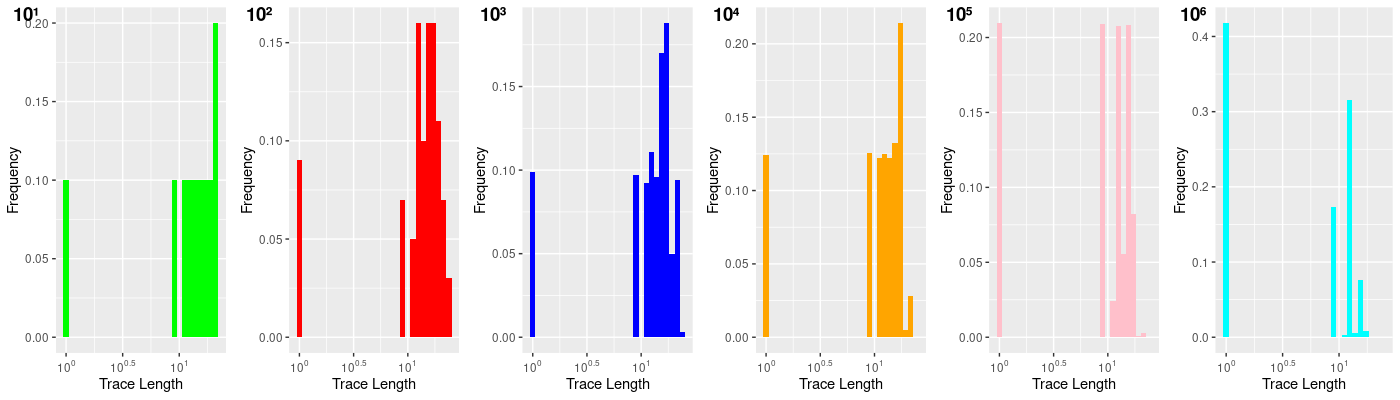
\includegraphics[width=\textwidth]{images/BrokerPDF.png}
\caption{FoodBroker dataset}\label{fbPDF}
\end{subfigure}
\begin{subfigure}{\textwidth}
\centering
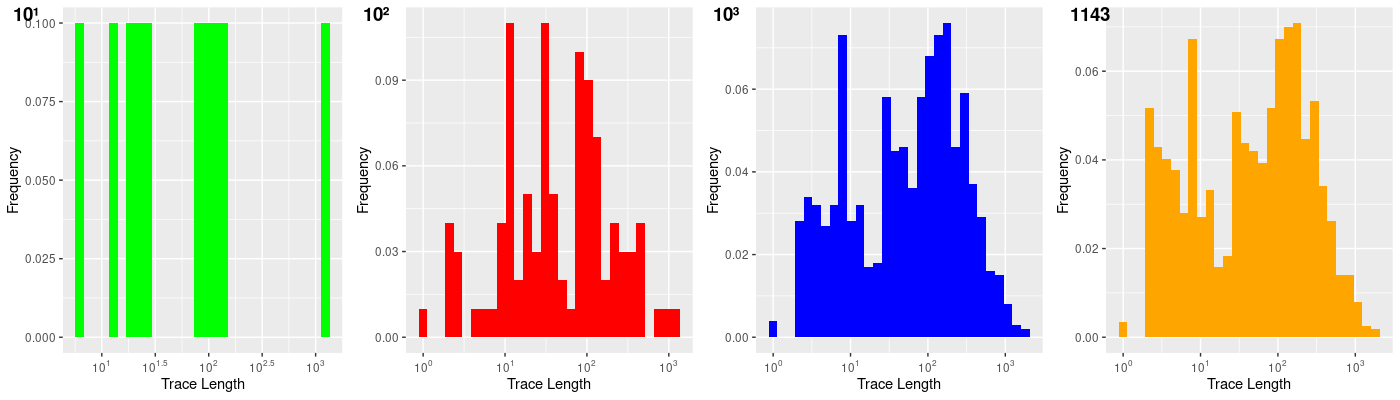
\includegraphics[width=\textwidth]{images/HospitalPDF.png}
\caption{Hospital dataset}\label{hPDF}
\end{subfigure}
\begin{subfigure}{\textwidth}
\centering
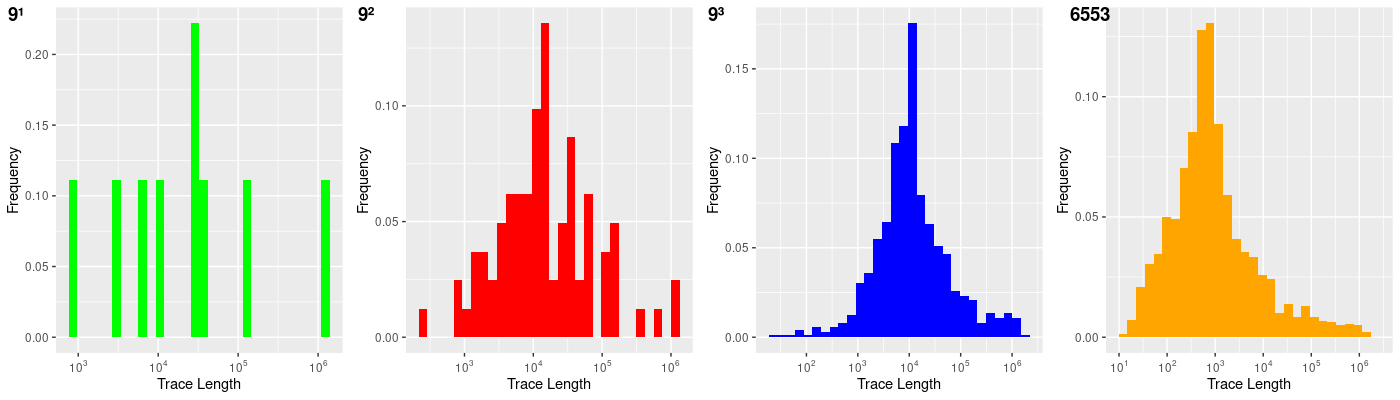
\includegraphics[width=\textwidth]{images/CyberPDF.png}
\caption{Cybersecurity dataset}\label{cPDF}
\end{subfigure}
\caption{Trace length sampled probability density over the sampled logs for the different datasets}\label{fig:PDF}
\end{figure*}\begin{figure*}[!p]
\centering
\begin{subfigure}{\textwidth}
\centering
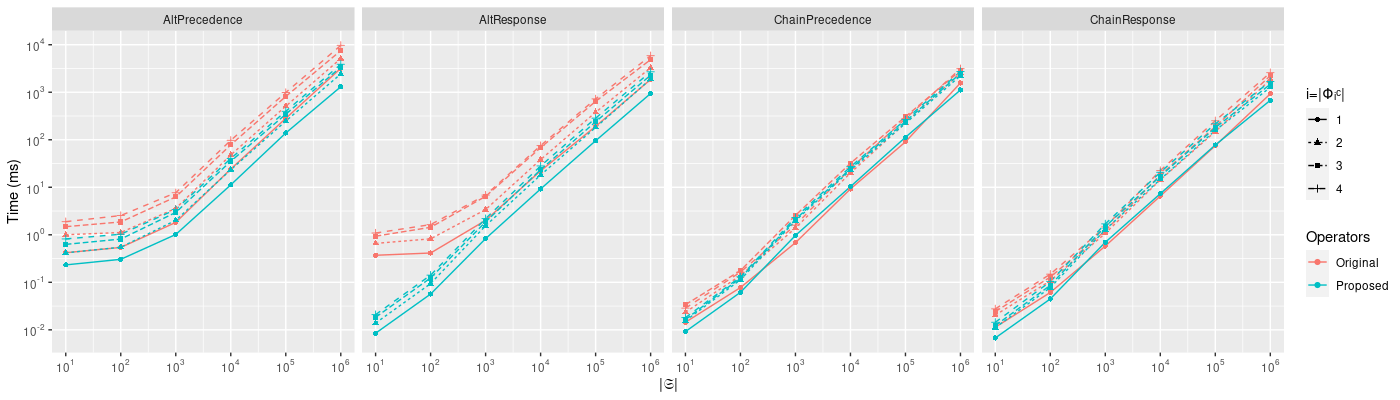
\includegraphics[width=\textwidth]{images/FoodBroker.png}
\caption{FoodBroker dataset}
\end{subfigure}
\begin{subfigure}{\textwidth}
\centering
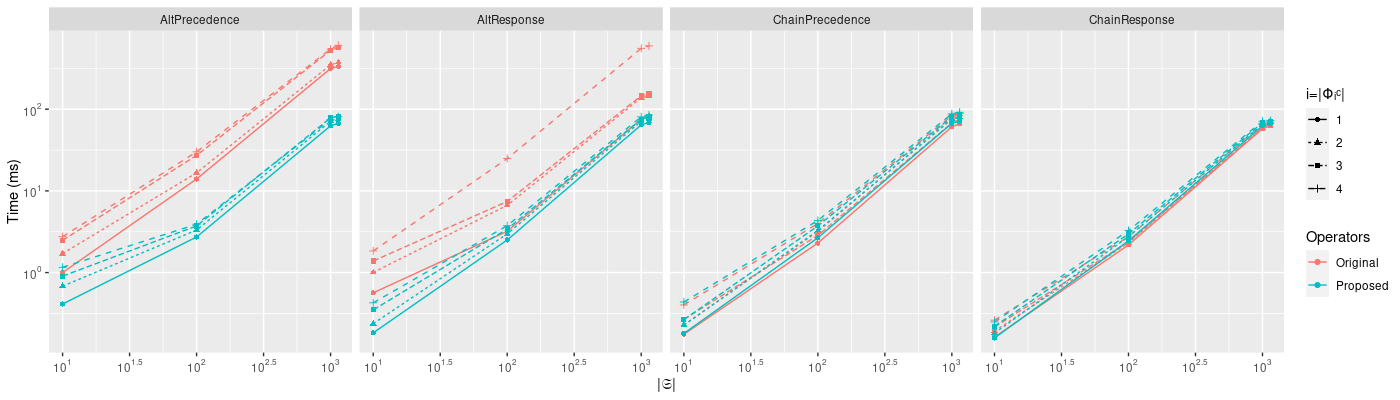
\includegraphics[width=\textwidth]{images/Hospital.png}
\caption{Hospital dataset}
\end{subfigure}
\begin{subfigure}{\textwidth}
\centering
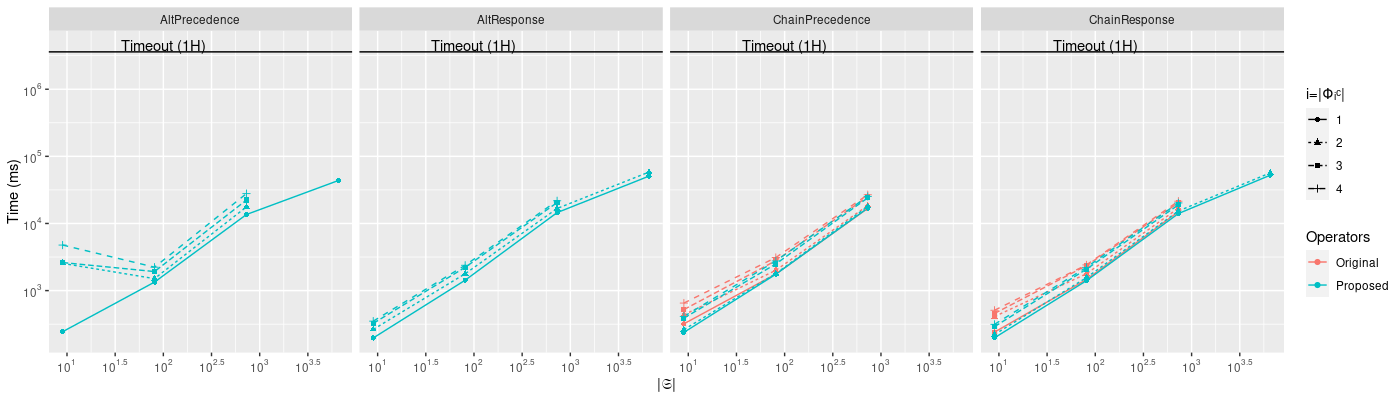
\includegraphics[width=\textwidth]{images/Cyber.png}
\caption{Cybersecurity dataset}
\end{subfigure}
\begin{subfigure}{\textwidth}
\centering
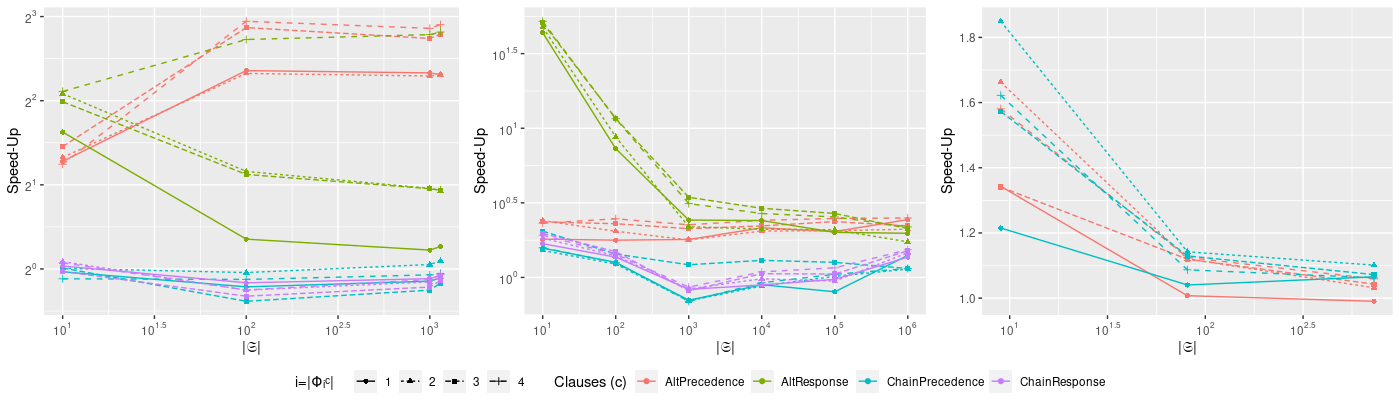
\includegraphics[width=\textwidth]{images/Speedups.png}
\caption{Datasets' Speedup: (\textit{left}) FoodBroker, (\textit{center}) Hospital, and (\textit{right}) Cybersecurity.}
\end{subfigure}
\caption{Comparing the proposed implementation of the derived operators with the previous implementation given in KnoBAB. }\label{overallBenchmarks}
\end{figure*}
For each dataset, we then obtain the sampled trace length distribution, and we sample sub-logs of various sizes while trying to abide by the trace distribution from the original dataset, notwithstanding the skewness of such distributions. For the first and third (or second) datasets we sample the logs so that their sizes are powers of ten (or nine) while always guaranteeing that each sub-log $|\LOG_h|=10^h$ (or $|\LOG_h|=9^h$) is always a subset of any larger sub-log. We also keep the original log as the last sample dataset. This random sampling mechanism is required to better assess the scalability of the proposed operator's implementation while guaranteeing an approximation of the original trace length distribution across the board, so as to guarantee similar running time conditions. \figurename~\ref{fig:PDF} reports the sample PDF trace length for each of the sampled logs alongside the size of each sample. We can observe that the \texttt{FoodBroker} synthetic dataset contains the shorter traces (\figurename~\ref{fbPDF}), where all the sampled logs except the first one have a maximum trace length of $24$, while the first sublog has a maximum trace length of $21$. On the other hand, the first two smaller log samples of the real-world \texttt{Hospital} dataset (\figurename~\ref{hPDF}) have traces with maximum length of $1200$, while the remaining two have a maximum trace length of $1814$. The \texttt{Cybersecurity} dataset (\figurename ~\ref{cPDF}) contains the longer traces by having the maximum trace length of $1.23\cdot10^6$ for the smaller two sub-logs and of $1.76\cdot 10^6$ for the remaining ones. This information will become soon relevant while conducting our following analysis over the algorithmic speed-ups given by our proposed derived operators while performing formal verification over the models described in the following paragraph.


 Given that our aim is to test these operator in the context of a Declare-based formal verification task when \texttt{xt}LTL\textsubscript{f} is used to represent its semantics, we generate four specifications $\Phi^c_1,\dots,\Phi^c_4$ for each declarative clause of interest $c$, \texttt{AltPrecedence}, \texttt{AltResponse}, \texttt{ChainPrecedence}, and \texttt{ChainResponse}, where each $\Phi^c_i$ contains exactly $i$ binary clauses instantiated by instantiating each activity label from the most frequently-occurring ones within the smaller sublog. We then use the same specifications being generated for the smaller log and also for the greater sublogs, thus comparing running experiments with the same specifications. The resulting logs and specifications are freely available online\footnote{\url{https://osf.io/6y8cv/?view_only=3b8c01761fcf4941ad726aba4101151e}}. \medskip

With reference to \figurename~\ref{overallBenchmarks}, Alt\ding{83} operators are the ones being more consistently outperforming our previous definition of the Declare semantics, as their associated speed-up is always strictly greater than zero. Our previous definition of the Declare operators is greatly affected by the number of the clauses within the model, which becomes even more apparent when the maximum and average trace length per sampled log increases. On the other hand, all the computations for such operators over the Cybersecurity dataset took more than one 1H ($3.6\cdot 10^6$ ms), thus remarking an increased running time for the original query plan strategy when longer traces occur. We stopped to record the running time, as the overhead introduced by the intermediate operators for carrying out the actual matching between activation and target conditions was more remarked, as our proposed operators could instead carry out the formal verification task within one minute of time. Despite no out-of-memory exceptions were observed before the timeout, these were clearly observed in larger specifications and log sizes, thus clearly remarking the limits of not persisting in secondary memory the query intermediate results. Despite the code allows to clear intermediate caches for freeing extra memory, these does not allow to cover all the possible specifications. Notwithstanding the former memory limitation concerns, this solution allows to return results within a reasonable amount of time. By given the original operators sufficient amount of time to compute, we also obtain similar out-of-memory errors. Overall, this remarks that this proposed extension for Alt\ding{83} operators outperform previous instantiations, as also expected from our previous analysis concerning the overall theoretical time complexity.


Chain\ding{83} operators provide a more convoluted scenario to examine carefully. First, we observe a clear trend correlating dataset with longer traces with an overall increase of speed-up. In fact, the \texttt{Hospital} datasets exhibits more speed-ups if compared to the \texttt{FoodBroker} one, where the recently-proposed operators yield to either comparable or underperforming performances. Notwithstanding the former, we can clearly observe that the recently-proposed operators consistently outperform our previous solution over the \texttt{Cybersecurity} dataset. Differently from our previous set-up, we can now observe that the original formulation of the declarative clauses without the currently-presented operators now goes out of memory before hitting the 1H timeout for the larger sample being the full dataset, while our solution still manages to carry out some temporal formal verification tasks over specifications containing fewer clauses. Last, we consistently observe that such operators still provide greater speed-ups over datasets with smaller log size, thus providing theoretical validation to our speed-up equations for such operators.


%\texttt{\color{red}[TODO: mainly discuss the experiments' outcome]}

\section{Conclusions and Future Works}
This paper proposes an extension to our previous work on KnoBAB by optimising the query plan induced by the exploitation of the relational temporal semantics \texttt{xt}LTL\textsubscript{f} for expressing temporal properties within the data. This is addressed through the definition of novel derived operators, that is, operators that can be expressed as combination of already-existing \texttt{xt}LTL\textsubscript{f} operators being a calque of the customary LTL\textsubscript{f} operators. Preliminary results that these operator show to lead the best speed-up in realistic use case scenarios where several events are audited and collected in a larger collection of traces.

Despite these experiments remark the efficiency of carrying out formal verification computations on columnar databases implemented as a main memory engine, the consistent out-of-memory faults that we experienced over larger collections of data containing more events (i.e., longer traces) encourage us to consider starting to port at least the intermediate result generation pipeline in secondary memory, as customary for off-the-shelf databases such as PostgreSQL. We see this as the last required step for fully-supporting real data alongside the orthogonal operator optimization as discussed in the present paper. 

The current experiment noted the optimality of the proposed operators when dealing with datasets with longer traces (i.e., greater $\epsilon$). Future work will consider the possibility of defining hybrid algorithms \cite{4567924} over the operators optimising Chain\ding{83} clauses  by empirically determining the table size threshold over which prefer the derived operators over the original. As an orthogonal approach, we will also define the ``dual'' operators for \texttt{AndNext} and \texttt{NextAnd} so to start scanning from the target condition while moving backwards towards any existing activation condition when the number of targets are deemed to be fewer than the activations. 

Our future works will be also aimed to further benchmark these operators in a context of \textit{dataful} logs, where events are also associated to a payload expressed as a key-value pair as in customary semi-structured data formats. These works will then outline the overhead required to compute a $\Theta$ correlation condition between activation and target event, which now contains no events. 

Finally, an interesting outcome of these observations on relational databases would be the application of such an algebra in the context of temporal graphs 
\cite{DBLP:conf/medi/ZakiHH022,DBLP:journals/vldb/RostGTFSCAJR22}, thus enabling the efficient temporal verification under this different data representation. 




%
%ACM's consolidated article template, introduced in 2017, provides a
%consistent \LaTeX\ style for use across ACM publications, and
%incorporates accessibility and metadata-extraction functionality
%necessary for future Digital Library endeavors. Numerous ACM and
%SIG-specific \LaTeX\ templates have been examined, and their unique
%features incorporated into this single new template.
%
%If you are new to publishing with ACM, this document is a valuable
%guide to the process of preparing your work for publication. If you
%have published with ACM before, this document provides insight and
%instruction into more recent changes to the article template.
%
%The ``\verb|acmart|'' document class can be used to prepare articles
%for any ACM publication --- conference or journal, and for any stage
%of publication, from review to final ``camera-ready'' copy, to the
%author's own version, with {\itshape very} few changes to the source.

%\section{Template Overview}
%As noted in the introduction, the ``\verb|acmart|'' document class can
%be used to prepare many different kinds of documentation --- a
%double-blind initial submission of a full-length technical paper, a
%two-page SIGGRAPH Emerging Technologies abstract, a ``camera-ready''
%journal article, a SIGCHI Extended Abstract, and more --- all by
%selecting the appropriate {\itshape template style} and {\itshape
%  template parameters}.
%
%This document will explain the major features of the document
%class. For further information, the {\itshape \LaTeX\ User's Guide} is
%available from
%\url{https://www.acm.org/publications/proceedings-template}.
%
%\subsection{Template Styles}
%
%The primary parameter given to the ``\verb|acmart|'' document class is
%the {\itshape template style} which corresponds to the kind of publication
%or SIG publishing the work. This parameter is enclosed in square
%brackets and is a part of the {\verb|documentclass|} command:
%\begin{verbatim}
%  \documentclass[STYLE]{acmart}
%\end{verbatim}
%
%Journals use one of three template styles. All but three ACM journals
%use the {\verb|acmsmall|} template style:
%\begin{itemize}
%\item {\texttt{acmsmall}}: The default journal template style.
%\item {\texttt{acmlarge}}: Used by JOCCH and TAP.
%\item {\texttt{acmtog}}: Used by TOG.
%\end{itemize}
%
%The majority of conference proceedings documentation will use the {\verb|acmconf|} template style.
%\begin{itemize}
%\item {\texttt{acmconf}}: The default proceedings template style.
%\item{\texttt{sigchi}}: Used for SIGCHI conference articles.
%\item{\texttt{sigplan}}: Used for SIGPLAN conference articles.
%\end{itemize}
%
%\subsection{Template Parameters}
%
%In addition to specifying the {\itshape template style} to be used in
%formatting your work, there are a number of {\itshape template parameters}
%which modify some part of the applied template style. A complete list
%of these parameters can be found in the {\itshape \LaTeX\ User's Guide.}
%
%Frequently-used parameters, or combinations of parameters, include:
%\begin{itemize}
%\item {\texttt{anonymous,review}}: Suitable for a ``double-blind''
%  conference submission. Anonymizes the work and includes line
%  numbers. Use with the \texttt{\acmSubmissionID} command to print the
%  submission's unique ID on each page of the work.
%\item{\texttt{authorversion}}: Produces a version of the work suitable
%  for posting by the author.
%\item{\texttt{screen}}: Produces colored hyperlinks.
%\end{itemize}
%
%This document uses the following string as the first command in the
%source file:
%\begin{verbatim}
%\documentclass[sigconf]{acmart}
%\end{verbatim}
%
%\section{Modifications}
%
%Modifying the template --- including but not limited to: adjusting
%margins, typeface sizes, line spacing, paragraph and list definitions,
%and the use of the \verb|\vspace| command to manually adjust the
%vertical spacing between elements of your work --- is not allowed.
%
%{\bfseries Your document will be returned to you for revision if
%  modifications are discovered.}
%
%\section{Typefaces}
%
%The ``\verb|acmart|'' document class requires the use of the
%``Libertine'' typeface family. Your \TeX\ installation should include
%this set of packages. Please do not substitute other typefaces. The
%``\verb|lmodern|'' and ``\verb|ltimes|'' packages should not be used,
%as they will override the built-in typeface families.
%
%\section{Title Information}
%
%The title of your work should use capital letters appropriately -
%\url{https://capitalizemytitle.com/} has useful rules for
%capitalization. Use the {\verb|title|} command to define the title of
%your work. If your work has a subtitle, define it with the
%{\verb|subtitle|} command.  Do not insert line breaks in your title.
%
%If your title is lengthy, you must define a short version to be used
%in the page headers, to prevent overlapping text. The \verb|title|
%command has a ``short title'' parameter:
%\begin{verbatim}
%  \title[short title]{full title}
%\end{verbatim}
%
%\section{Authors and Affiliations}
%
%Each author must be defined separately for accurate metadata
%identification.  As an exception, multiple authors may share one
%affiliation. Authors' names should not be abbreviated; use full first
%names wherever possible. Include authors' e-mail addresses whenever
%possible.
%
%Grouping authors' names or e-mail addresses, or providing an ``e-mail
%alias,'' as shown below, is not acceptable:
%\begin{verbatim}
%  \author{Brooke Aster, David Mehldau}
%  \email{dave,judy,steve@university.edu}
%  \email{firstname.lastname@phillips.org}
%\end{verbatim}
%
%The \verb|authornote| and \verb|authornotemark| commands allow a note
%to apply to multiple authors --- for example, if the first two authors
%of an article contributed equally to the work.
%
%If your author list is lengthy, you must define a shortened version of
%the list of authors to be used in the page headers, to prevent
%overlapping text. The following command should be placed just after
%the last \verb|\author{}| definition:
%\begin{verbatim}
%  \renewcommand{\shortauthors}{McCartney, et al.}
%\end{verbatim}
%Omitting this command will force the use of a concatenated list of all
%of the authors' names, which may result in overlapping text in the
%page headers.
%
%The article template's documentation, available at
%\url{https://www.acm.org/publications/proceedings-template}, has a
%complete explanation of these commands and tips for their effective
%use.
%
%Note that authors' addresses are mandatory for journal articles.
%
%\section{Rights Information}
%
%Authors of any work published by ACM will need to complete a rights
%form. Depending on the kind of work, and the rights management choice
%made by the author, this may be copyright transfer, permission,
%license, or an OA (open access) agreement.
%
%Regardless of the rights management choice, the author will receive a
%copy of the completed rights form once it has been submitted. This
%form contains \LaTeX\ commands that must be copied into the source
%document. When the document source is compiled, these commands and
%their parameters add formatted text to several areas of the final
%document:
%\begin{itemize}
%\item the ``ACM Reference Format'' text on the first page.
%\item the ``rights management'' text on the first page.
%\item the conference information in the page header(s).
%\end{itemize}
%
%Rights information is unique to the work; if you are preparing several
%works for an event, make sure to use the correct set of commands with
%each of the works.
%
%The ACM Reference Format text is required for all articles over one
%page in length, and is optional for one-page articles (abstracts).
%
%\section{CCS Concepts and User-Defined Keywords}
%
%Two elements of the ``acmart'' document class provide powerful
%taxonomic tools for you to help readers find your work in an online
%search.
%
%The ACM Computing Classification System ---
%\url{https://www.acm.org/publications/class-2012} --- is a set of
%classifiers and concepts that describe the computing
%discipline. Authors can select entries from this classification
%system, via \url{https://dl.acm.org/ccs/ccs.cfm}, and generate the
%commands to be included in the \LaTeX\ source.
%
%User-defined keywords are a comma-separated list of words and phrases
%of the authors' choosing, providing a more flexible way of describing
%the research being presented.
%
%CCS concepts and user-defined keywords are required for for all
%articles over two pages in length, and are optional for one- and
%two-page articles (or abstracts).
%
%\section{Sectioning Commands}
%
%Your work should use standard \LaTeX\ sectioning commands:
%\verb|section|, \verb|subsection|, \verb|subsubsection|, and
%\verb|paragraph|. They should be numbered; do not remove the numbering
%from the commands.
%
%Simulating a sectioning command by setting the first word or words of
%a paragraph in boldface or italicized text is {\bfseries not allowed.}
%
%\section{Tables}
%
%The ``\verb|acmart|'' document class includes the ``\verb|booktabs|''
%package --- \url{https://ctan.org/pkg/booktabs} --- for preparing
%high-quality tables.
%
%Table captions are placed {\itshape above} the table.
%
%Because tables cannot be split across pages, the best placement for
%them is typically the top of the page nearest their initial cite.  To
%ensure this proper ``floating'' placement of tables, use the
%environment \textbf{table} to enclose the table's contents and the
%table caption.  The contents of the table itself must go in the
%\textbf{tabular} environment, to be aligned properly in rows and
%columns, with the desired horizontal and vertical rules.  Again,
%detailed instructions on \textbf{tabular} material are found in the
%\textit{\LaTeX\ User's Guide}.
%
%Immediately following this sentence is the point at which
%Table~\ref{tab:freq} is included in the input file; compare the
%placement of the table here with the table in the printed output of
%this document.
%
%\begin{table}
%  \caption{Frequency of Special Characters}
%  \label{tab:freq}
%  \begin{tabular}{ccl}
%    \toprule
%    Non-English or Math&Frequency&Comments\\
%    \midrule
%    \O & 1 in 1,000& For Swedish names\\
%    $\pi$ & 1 in 5& Common in math\\
%    \$ & 4 in 5 & Used in business\\
%    $\Psi^2_1$ & 1 in 40,000& Unexplained usage\\
%  \bottomrule
%\end{tabular}
%\end{table}
%
%To set a wider table, which takes up the whole width of the page's
%live area, use the environment \textbf{table*} to enclose the table's
%contents and the table caption.  As with a single-column table, this
%wide table will ``float'' to a location deemed more
%desirable. Immediately following this sentence is the point at which
%Table~\ref{tab:commands} is included in the input file; again, it is
%instructive to compare the placement of the table here with the table
%in the printed output of this document.
%
%\begin{table*}
%  \caption{Some Typical Commands}
%  \label{tab:commands}
%  \begin{tabular}{ccl}
%    \toprule
%    Command &A Number & Comments\\
%    \midrule
%    \texttt{{\char'134}author} & 100& Author \\
%    \texttt{{\char'134}table}& 300 & For tables\\
%    \texttt{{\char'134}table*}& 400& For wider tables\\
%    \bottomrule
%  \end{tabular}
%\end{table*}
%
%Always use midrule to separate table header rows from data rows, and
%use it only for this purpose. This enables assistive technologies to
%recognise table headers and support their users in navigating tables
%more easily.
%
%\section{Math Equations}
%You may want to display math equations in three distinct styles:
%inline, numbered or non-numbered display.  Each of the three are
%discussed in the next sections.
%
%\subsection{Inline (In-text) Equations}
%A formula that appears in the running text is called an inline or
%in-text formula.  It is produced by the \textbf{math} environment,
%which can be invoked with the usual
%\texttt{{\char'134}begin\,\ldots{\char'134}end} construction or with
%the short form \texttt{\$\,\ldots\$}. You can use any of the symbols
%and structures, from $\alpha$ to $\omega$, available in
%\LaTeX~\cite{Lamport:LaTeX}; this section will simply show a few
%examples of in-text equations in context. Notice how this equation:
%\begin{math}
%  \lim_{n\rightarrow \infty}x=0
%\end{math},
%set here in in-line math style, looks slightly different when
%set in display style.  (See next section).
%
%\subsection{Display Equations}
%A numbered display equation---one set off by vertical space from the
%text and centered horizontally---is produced by the \textbf{equation}
%environment. An unnumbered display equation is produced by the
%\textbf{displaymath} environment.
%
%Again, in either environment, you can use any of the symbols and
%structures available in \LaTeX\@; this section will just give a couple
%of examples of display equations in context.  First, consider the
%equation, shown as an inline equation above:
%\begin{equation}
%  \lim_{n\rightarrow \infty}x=0
%\end{equation}
%Notice how it is formatted somewhat differently in
%the \textbf{displaymath}
%environment.  Now, we'll enter an unnumbered equation:
%\begin{displaymath}
%  \sum_{i=0}^{\infty} x + 1
%\end{displaymath}
%and follow it with another numbered equation:
%\begin{equation}
%  \sum_{i=0}^{\infty}x_i=\int_{0}^{\pi+2} f
%\end{equation}
%just to demonstrate \LaTeX's able handling of numbering.
%
%\section{Figures}
%
%The ``\verb|figure|'' environment should be used for figures. One or
%more images can be placed within a figure. If your figure contains
%third-party material, you must clearly identify it as such, as shown
%in the example below.
%%\begin{figure}[h]
%%  \centering
%%  \includegraphics[width=\linewidth]{sample-franklin}
%%  \caption{1907 Franklin Model D roadster. Photograph by Harris \&
%%    Ewing, Inc. [Public domain], via Wikimedia
%%    Commons. (\url{https://goo.gl/VLCRBB}).}
%%  \Description{A woman and a girl in white dresses sit in an open car.}
%%\end{figure}
%
%Your figures should contain a caption which describes the figure to
%the reader.
%
%Figure captions are placed {\itshape below} the figure.
%
%Every figure should also have a figure description unless it is purely
%decorative. These descriptions convey what’s in the image to someone
%who cannot see it. They are also used by search engine crawlers for
%indexing images, and when images cannot be loaded.
%
%A figure description must be unformatted plain text less than 2000
%characters long (including spaces).  {\bfseries Figure descriptions
%  should not repeat the figure caption – their purpose is to capture
%  important information that is not already provided in the caption or
%  the main text of the paper.} For figures that convey important and
%complex new information, a short text description may not be
%adequate. More complex alternative descriptions can be placed in an
%appendix and referenced in a short figure description. For example,
%provide a data table capturing the information in a bar chart, or a
%structured list representing a graph.  For additional information
%regarding how best to write figure descriptions and why doing this is
%so important, please see
%\url{https://www.acm.org/publications/taps/describing-figures/}.
%
%\subsection{The ``Teaser Figure''}
%
%A ``teaser figure'' is an image, or set of images in one figure, that
%are placed after all author and affiliation information, and before
%the body of the article, spanning the page. If you wish to have such a
%figure in your article, place the command immediately before the
%\verb|\maketitle| command:
%\begin{verbatim}
%  \begin{teaserfigure}
%    \includegraphics[width=\textwidth]{sampleteaser}
%    \caption{figure caption}
%    \Description{figure description}
%  \end{teaserfigure}
%\end{verbatim}
%
%\section{Citations and Bibliographies}
%
%The use of \BibTeX\ for the preparation and formatting of one's
%references is strongly recommended. Authors' names should be complete
%--- use full first names (``Donald E. Knuth'') not initials
%(``D. E. Knuth'') --- and the salient identifying features of a
%reference should be included: title, year, volume, number, pages,
%article DOI, etc.
%
%The bibliography is included in your source document with these two
%commands, placed just before the \verb|\end{document}| command:
%\begin{verbatim}
%  \bibliographystyle{ACM-Reference-Format}
%  \bibliography{bibfile}
%\end{verbatim}
%where ``\verb|bibfile|'' is the name, without the ``\verb|.bib|''
%suffix, of the \BibTeX\ file.
%
%Citations and references are numbered by default. A small number of
%ACM publications have citations and references formatted in the
%``author year'' style; for these exceptions, please include this
%command in the {\bfseries preamble} (before the command
%``\verb|\begin{document}|'') of your \LaTeX\ source:
%\begin{verbatim}
%  \citestyle{acmauthoryear}
%\end{verbatim}
%
%
%  Some examples.  A paginated journal article \cite{Abril07}, an
%  enumerated journal article \cite{Cohen07}, a reference to an entire
%  issue \cite{JCohen96}, a monograph (whole book) \cite{Kosiur01}, a
%  monograph/whole book in a series (see 2a in spec. document)
%  \cite{Harel79}, a divisible-book such as an anthology or compilation
%  \cite{Editor00} followed by the same example, however we only output
%  the series if the volume number is given \cite{Editor00a} (so
%  Editor00a's series should NOT be present since it has no vol. no.),
%  a chapter in a divisible book \cite{Spector90}, a chapter in a
%  divisible book in a series \cite{Douglass98}, a multi-volume work as
%  book \cite{Knuth97}, a couple of articles in a proceedings (of a
%  conference, symposium, workshop for example) (paginated proceedings
%  article) \cite{Andler79, Hagerup1993}, a proceedings article with
%  all possible elements \cite{Smith10}, an example of an enumerated
%  proceedings article \cite{VanGundy07}, an informally published work
%  \cite{Harel78}, a couple of preprints \cite{Bornmann2019,
%    AnzarootPBM14}, a doctoral dissertation \cite{Clarkson85}, a
%  master's thesis: \cite{anisi03}, an online document / world wide web
%  resource \cite{Thornburg01, Ablamowicz07, Poker06}, a video game
%  (Case 1) \cite{Obama08} and (Case 2) \cite{Novak03} and \cite{Lee05}
%  and (Case 3) a patent \cite{JoeScientist001}, work accepted for
%  publication \cite{rous08}, 'YYYYb'-test for prolific author
%  \cite{SaeediMEJ10} and \cite{SaeediJETC10}. Other cites might
%  contain 'duplicate' DOI and URLs (some SIAM articles)
%  \cite{Kirschmer:2010:AEI:1958016.1958018}. Boris / Barbara Beeton:
%  multi-volume works as books \cite{MR781536} and \cite{MR781537}. A
%  couple of citations with DOIs:
%  \cite{2004:ITE:1009386.1010128,Kirschmer:2010:AEI:1958016.1958018}. Online
%  citations: \cite{TUGInstmem, Thornburg01, CTANacmart}.
%  Artifacts: \cite{R} and \cite{UMassCitations}.
%
%\section{Acknowledgments}
%
%Identification of funding sources and other support, and thanks to
%individuals and groups that assisted in the research and the
%preparation of the work should be included in an acknowledgment
%section, which is placed just before the reference section in your
%document.
%
%This section has a special environment:
%\begin{verbatim}
%  \begin{acks}
%  ...
%  \end{acks}
%\end{verbatim}
%so that the information contained therein can be more easily collected
%during the article metadata extraction phase, and to ensure
%consistency in the spelling of the section heading.
%
%Authors should not prepare this section as a numbered or unnumbered {\verb|\section|}; please use the ``{\verb|acks|}'' environment.
%
%\section{Appendices}
%
%If your work needs an appendix, add it before the
%``\verb|\end{document}|'' command at the conclusion of your source
%document.
%
%Start the appendix with the ``\verb|appendix|'' command:
%\begin{verbatim}
%  \appendix
%\end{verbatim}
%and note that in the appendix, sections are lettered, not
%numbered. This document has two appendices, demonstrating the section
%and subsection identification method.
%
%\section{Multi-language papers}
%
%Papers may be written in languages other than English or include
%titles, subtitles, keywords and abstracts in different languages (as a
%rule, a paper in a language other than English should include an
%English title and an English abstract).  Use \verb|language=...| for
%every language used in the paper.  The last language indicated is the
%main language of the paper.  For example, a French paper with
%additional titles and abstracts in English and German may start with
%the following command
%\begin{verbatim}
%\documentclass[sigconf, language=english, language=german,
%               language=french]{acmart}
%\end{verbatim}
%
%The title, subtitle, keywords and abstract will be typeset in the main
%language of the paper.  The commands \verb|\translatedXXX|, \verb|XXX|
%begin title, subtitle and keywords, can be used to set these elements
%in the other languages.  The environment \verb|translatedabstract| is
%used to set the translation of the abstract.  These commands and
%environment have a mandatory first argument: the language of the
%second argument.  See \verb|sample-sigconf-i13n.tex| file for examples
%of their usage.
%
%\section{SIGCHI Extended Abstracts}
%
%The ``\verb|sigchi-a|'' template style (available only in \LaTeX\ and
%not in Word) produces a landscape-orientation formatted article, with
%a wide left margin. Three environments are available for use with the
%``\verb|sigchi-a|'' template style, and produce formatted output in
%the margin:
%\begin{description}
%\item[\texttt{sidebar}:]  Place formatted text in the margin.
%\item[\texttt{marginfigure}:] Place a figure in the margin.
%\item[\texttt{margintable}:] Place a table in the margin.
%\end{description}
%
%%%
%%% The acknowledgments section is defined using the "acks" environment
%%% (and NOT an unnumbered section). This ensures the proper
%%% identification of the section in the article metadata, and the
%%% consistent spelling of the heading.
%\begin{acks}
%To Robert, for the bagels and explaining CMYK and color spaces.
%\end{acks}
%
%%%
%%% The next two lines define the bibliography style to be used, and
%%% the bibliography file.

\bibliographystyle{ACM-Reference-Format}
\bibliography{refs}

%
%%%
%%% If your work has an appendix, this is the place to put it.
%\appendix
%
%\section{Research Methods}
%
%\subsection{Part One}
%
%Lorem ipsum dolor sit amet, consectetur adipiscing elit. Morbi
%malesuada, quam in pulvinar varius, metus nunc fermentum urna, id
%sollicitudin purus odio sit amet enim. Aliquam ullamcorper eu ipsum
%vel mollis. Curabitur quis dictum nisl. Phasellus vel semper risus, et
%lacinia dolor. Integer ultricies commodo sem nec semper.
%
%\subsection{Part Two}
%
%Etiam commodo feugiat nisl pulvinar pellentesque. Etiam auctor sodales
%ligula, non varius nibh pulvinar semper. Suspendisse nec lectus non
%ipsum convallis congue hendrerit vitae sapien. Donec at laoreet
%eros. Vivamus non purus placerat, scelerisque diam eu, cursus
%ante. Etiam aliquam tortor auctor efficitur mattis.
%
%\section{Online Resources}
%
%Nam id fermentum dui. Suspendisse sagittis tortor a nulla mollis, in
%pulvinar ex pretium. Sed interdum orci quis metus euismod, et sagittis
%enim maximus. Vestibulum gravida massa ut felis suscipit
%congue. Quisque mattis elit a risus ultrices commodo venenatis eget
%dui. Etiam sagittis eleifend elementum.
%
%Nam interdum magna at lectus dignissim, ac dignissim lorem
%rhoncus. Maecenas eu arcu ac neque placerat aliquam. Nunc pulvinar
%massa et mattis lacinia.

\end{document}
\endinput
%%
%% End of file `sample-sigconf.tex'.

